% Тут используется класс, установленный на сервере Papeeria. На случай, если
% текст понадобится редактировать где-то в другом месте, рядом лежит файл matmex-diploma-custom.cls
% который в момент своего создания был идентичен классу, установленному на сервере.
% Для того, чтобы им воспользоваться, замените matmex-diploma на matmex-diploma-custom
% Если вы работаете исключительно в Papeeria то мы настоятельно рекомендуем пользоваться
% классом matmex-diploma, поскольку он будет автоматически обновляться по мере внесения корректив
%

% По умолчанию используется шрифт 14 размера. Если нужен 12-й шрифт, уберите опцию [14pt]
%\documentclass[14pt]{matmex-diploma}
\documentclass{matmex-diploma-custom}

\linespread{1.0}
\begin{document}
% Год, город, название университета и факультета предопределены,
% но можно и поменять.
% Если англоязычная титульная страница не нужна, то ее можно просто удалить.
\filltitle{ru}{
    chair              = {Кафедра небесной механики},
    title              = {Пространственно-кинематическое моделирование плоской подсистемы Галактики},
    % Здесь указывается тип работы. Возможные значения:
    %   coursework - Курсовая работа
    %   diploma - Диплом специалиста
    %   master - Диплом магистра
    %   bachelor - Диплом бакалавра
    type               = {diploma},
    position           = {студента},
    group              = 666,
    author             = {Волков Даниил Валентинович},
    supervisorPosition = {к.\,ф.-м.\,н., доцент},
    supervisor         = {Никифоров И.\,И.\\ Кафедра небесной механики},
    reviewerPosition   = {к.\,ф.-м.\,н., старший научный сотрудник},
    reviewer           = {Мосенков А.\,В. \\ ГАО РАН},
    chairHeadPosition  = {д.\,ф.-м.\,н., профессор},
    chairHead          = {Холшевников К.\,В.},
%   university         = {Санкт-Петербургский Государственный Университет},
    faculty            = {Математико-механический факультет},
%   city               = {Санкт-Петербург},
%   year               = {2013}
}
\filltitle{en}{
    chair              = {Chair of Celestial Mechanics},
    title              = {Modeling of the flat subsystem \\ of the Milky Way},
    author             = {Daniil Volkov},
    supervisorPosition = {professor},
    supervisor         = {Igor Nikiforov},
    reviewerPosition   = {assistant},
    reviewer           = {Alexander Mosenkov},
    chairHeadPosition  = {professor},
    chairHead          = {Коnstantin Kholshevnikov},
}
\maketitle
\tableofcontents
% У введения нет номера главы
\section*{Введение}
Настоящая дипломная работа посвящена моделированию галактической кинематики совместно с установлением масштабного параметра -- расстояния от Солнца до центра Галактики $R_0$. Кинематическое моделирование подразумевает нахождение оценок для таких важных характеристик Галактики, как постоянная Оорта $A$, инвариант $AR_0$, линейная скорость вращения на солнечном круге $\theta_0$, кривая вращения Галактики. Несмотря на то, что проблеме определения $R_0$ уже очень много лет (первые оценки были сделаны Shapley ещё в 1918 году \cite{7}), усовершенствование имеющихся и разработка новых методов определения $R_0$ является актуальной задачей и по сей день, так как решение многих вопросов галактической и внегалактической астрономии и астрофизики требует знания упомянутых характеристик Галактики. Здесь приведен список конкретных задач и направлений исследований, зависящие от этих характеристик \cite{8}. В частности, от значения $R_0$ зависят 
\begin{itemize}
        \item абсолютный размер Галактики и её светимость,
        \item величина $\theta_0$,
        \item кривая вращения Галактики (зависимость линейной скорости $\theta$ от абсолютного галактоцентрического расстояния $R$),
        \item кинематические гелиоцентрические расстояния до галактических объектов, определяемые по принятому закону вращения Галактики (например, для планетарных туманностей \cite{4}),
        \item калибровка шкал расстояний до галактических объектов, для которых калибровки абсолютными методами по близким объектам менее точны или невозможны (планетарные туманности балджа \cite{12} и диска \cite{11}),
        \item понимание природы галактического центра: размеры, светимость, масса центральной части,
        \item внегалактические расстояния через перекалибровку абсолютных величин переменных типа классических цефеид, шаровых скоплений, RR Лиры и как результат постоянная Хаббла, возраст Вселенной и размеры её видимой части. 
\end{itemize}
\par От значения $\theta_0$ зависят вид галактической кривой вращения (относительно небольшие изменения этого параметра делают кривую вращения либо в среднем убывающей, либо плоской, либо возрастающей -- что сильно влияет на динамические выводы (ср., например, \cite{17}, \cite{18}, \cite{19})), проблема <<темной материи>> в Местной группе галактик (через приведение к центру Млечного Пути наблюдаемых скоростей в Местной группе), исследования распределения масс по локальным отклонениям от закона Хаббла.
\par Кривая вращения нужна для определения кинематических расстояний до объектов (при заданном $R_0$), исследования распределения масс в Галактике, моделирования динамических эффектов, возмущающих осесимметричное вращение (например, исследования спиральной структуры по кинематическим проявлениям волн плотности \cite{20}, \cite{21}, \cite{22}).
\par Так как параметры $A$ и $AR_0$ суть параметры закона вращения, то они влияют на те же задачи, что и сам закон вращения. Но помимо этого, они нужны для того, чтобы косвенно найти другие галактические параметры -- скорость вращения Галактики $\theta_0$ по наблюдаемому отношению радиальной и тангенциальной дисперсий остаточных скоростей \cite{23}, плотность вещества в окресностях Солнца \cite{24}. 
\par Получение величины остаточного движения позволяет выполнить более точное кинематическое моделирование, а также влияет на определение радиуса коротации в Галактике \cite{25}.
\par Выводом вышеуказанного является то, что проблемы моделирования тесно взаимосвязаны. Однако, в большом количестве они рассматриваются изолировано, в частности, необоснованно используются результаты других исследований. 
\par \textbf{Цель} данной работы -- выполнить пространственно-кинематическое моделирование Галактики по данным о плоской подсистеме, учитывая слабые стороны традиционных подходов. Рассматриваемые опорные объекты -- звезды красного сгущения (далее ЗКС) -- это высокометалличный аналог горизонтальной ветви, состоящий из населения II типа. Пачыньски и Станек (\cite{26}, \cite{27}) выдвинули звезды красного сгущения как новый индикатор расстояний и использовали эти звезды как опорные объекты для опредления $R_0$ методом Бааде. Преимущество этих звезд как опорных объектов -- в их многочисленности, что дает высокую статистическую точность оценки $R_0$. Используемый каталог APOGEE-RC \cite{2} содержит более 29 тыс. объектов c очень точными данными о лучевых скоростях. 
\par В настоящей работе к этим опорным объектам применяется трехкомпонентная кинематическая модель -- то есть, включаются данные и о лучевых скоростях, и о собственных движениях. Полностью определено воспроизведение конечной выборки, по которой получается решение. Кроме того, в отличии от многих подобных работ в этой области, здесь оптимизируется и порядок модели (модельных полиномов), а также применяется гибкий алгоритм исключения из выборки объектов с большими невязками.

\par 
\section{Пространственно-кинематическое моделирование плоской подсистемы}

Для кинематических методов определения $R_0$ характерна проблема зависимости результата от модельных и оптимизационных предположений. Поэтому подойти к их выбору следует максимально аккуратно.
\subsection{Основные предположения и определения}
Кинематическая модель должна описывать дифференциальное вращение Галактики, и стандартно его полагают осесимметричным.

\textbf{Предположение 1.}
Зависимость линейной скорости $\Theta$ движения подсистем Галактики -- это функция галактоосевого расстояния $R$: 
\begin{equation}
        \Theta = \Theta(R).
\end{equation}

На явлении вращения и основан кинематический метод определения $R_0$, имеющей в этом случае смысл расстояния до среднего центра кривизны линий равной скорости вращения. Т.к. центр может быть локализован по небольшой дуге окружности, не обязательно иметь данные, представляющие все галактические долготы, и такая неполнота исходных данных не является источником систематических ошибок.
\par Кроме обязательной вращательной составляющей модель может включать также представления и других эффектов галактической кинематики, в том числе о движении Солнца относительно Местного Стандарта Покоя. Так как каталожные лучевые скорости не приведены к МСП, то мы включаем остаточное движение Солнца как параметр модели. 

\textbf{Предположение 2.}
Компоненты остаточного движения Солнца относительно ВСП: $u_{\odot}, v_{\odot}, w_{\odot}$ предполагаются заранее неизвестными и находятся вместе с другими параметрами модели из той же самой выборки.

\par $K$-член (член Кемпбелла) -- эмпирическая постоянная добавка в уравнениях для лучевой скорости, отражающая влияние факторов, могущих вызвать дополнительное смещение спектральных линий \cite{3}. Во некоторых работах (напр., \cite{28} \cite{29}) используется как один из параметров модели. Однако большинство работ выявляет, что ошибка при определении этого параметра превышает найденные точечные оценки, поэтому от добавления его в модель в данной работе воздержались.

\textbf{Предположение 3.}
$K = 0$.

\par Другой возможный источник предположений -- вид представления закона дифференциального вращения. В подавляющем большинстве работ, посвященных проблеме $R_0$, фиксировалась аналитическая форма закона вращения (см., например, \cite{28}, \cite{30}, \cite{31}). В данной работе производится оптимизация аналитической формы и параметров закона вращения. Под оптимизацией формы понимается объективно обоснованный выбор из некоторого множества моделей такого их подмножества, что смещения $R_0$ из-за систематических ошибок аппроксимации -- наименьшие. При представлении закона вращения разложением в ряд оптимизацией формы будем называть оптимизацию порядка аппроксимирующего полинома. В нашем случае учет членов высоких порядков осмыслен, т.к. данные об опорных объектах покрывают значительный промежуток $R$.

\textbf{Предположение 4.}
Порядок разложения $n$ считается заранее неизвестным и оптимизируется в ходе решения.

Метод поиска параметров модели исходит из некоторых предположений о характере отклонений измеряемых величин от модельных предсказаний. Эти отклонения обычно принимаются распределенными по нормальному закону с нулевым математическим ожиданием, что даёт право применять метод наименьших квадратов (МНК).

\textbf{Предположение 5.}
Невязки (отклонения) наблюдаемых от модельных скоростей распределены по нормальному закону с нулевым математическим ожиданием: 
\begin{equation}
        \delta_{V_{\mathrm{mod}}, V_{\mathrm{obs}}} \in \mathcal{N}(0, \sigma^2_{V_{\mathrm{mod}}})
\end{equation}


Также стоить уточнить определение кривой вращения, которым мы будем пользоваться. \textit{Кривая вращения} -- зависимость от $R$ средней скорости вращения рассматриваемой подсистемы Галактики. Усреднение проводится и по галактической долготе, и по $Z$. Именно в таком смысле следует понимать кривые вращения, которые находятся из наблюдаемых данных. Говорить о кривой вращения как о зависимости от $R$ круговой скорости вращения в плоскости Галактики в данном случае нельзя из-за высокой дисперсии скоростей опорных объектов. Отметим также, что на кривую вращения влияет радиальный градиент металличности в Галактике (\cite{13}, \cite{14}), из-за которого может быть некорректным применение одинаковой калибровки к опорным объектам, находящимся на разных $R$. 

\textit{Модельная скорость} заданного объекта -- скорость центроида объектов данного типа, вычисленная для положения этого объекта.

\textit{Вращательный стандарт покоя} (ВСП) -- гелиоцентрическая система отсчета, движущаяся по круговой орбите со скоростью равной средней скорости вращения рассматриваемой подсистемы на $R = R_0$.

%Вклад в модельную скорость вращения подсистемы -- $V_{\mathrm{rot}}$.

%Вклад в модельную скорость движения Солнца относительно ВСП подсистемы -- $V_{\odot}$.


\subsection{Кинематическая модель}

В предположении кругового движения модельная лучевая скорость объекта относительно МСП определяется выражением \cite{3}
\begin{equation}
        V_{\mathrm{mod}} = (\omega - \omega_0) R_0 \sin{l} \cos{b} - V_{r, \odot},
\end{equation}
где $\omega$ и $\omega_0$ -- угловые скорости вращения подсистемы на $R$ и $R_0$, $l$ -- галактическая долгота, $b$ -- галактическая широта, $r$ -- гелиоцентрическое расстояние, $V_{r, \odot}$ -- проекция остаточной скорости движения Солнца.

Aналогично для собственных движений \cite{3}
\begin{equation}
        \mu_{l, \mathrm{mod}} = (\omega - \omega_0) \left( \frac{R_0\cos{l}}{r} - \cos{b} \right) - \omega_0 \cos{b} + \mu_{l, \odot},
\end{equation}
\begin{equation}
        \mu_{b, \mathrm{mod}} = - (\omega - \omega_0) \frac{R_0}{r} \sin{l} \sin{b} + \mu_{b, \odot}.
\end{equation}

\par Для представления кривой вращения $\Theta(R)$ используем модельный полином в виде многочлена Тейлора:
\begin{equation} \label{theta_n}
        \Theta_n(R)=\sum _{i=0}^{n} \frac{d^i\Theta \cdot (R - R_0)^i}{dR^i\cdot i!}.
\end{equation}
Галактоосевое расстояние $R$ определяется как \cite{3}
\begin{equation}
	R = \sqrt{R_0^2 + r^2 \cos^2{b} - 2R_0 r \cos{l} \cos{b}}.
\end{equation}

\par В качестве модели закона вращения выбрано разложение для линейной, а не угловой скорости, так как кривые вращения внешних спиральных Галактик и нашей Галактики плоские в первом приближении, и нелинейные члены (\ref{theta_n}) непосредственно описывают отклонения от этой простой модели, а в случае разложения в ряд $\omega(R)$ даже при плоской кривой вращения новые нелинейные члены будут требоваться просто по мере увеличения промежутка $\Delta R$, т.к. $\omega(R) \propto R^{-1}$.

\par Итак, получаем следующие рассчетные формулы для модельных скоростей опорных объектов.

\subsubsection{Лучевые скорости} \label{def_mod_vr}
\begin{equation}
        V_{r, \mathrm{rot}} = (\omega - \omega_0)R_0 \sin{l} \cos{b},
\end{equation}
\begin{equation}
        V_{r, \odot} = -u_{\odot} \cos{l} \cos{b} - v_{\odot} \cos{b} \sin{l} - w_{\odot} \sin{b}.
\end{equation}

\begin{equation}
        V_{r, \mathrm{mod}} = \left[ -2A\Delta R + \sum^n_{k = 2} \frac{\theta_k}{k!} \left( \Delta R \right)^k \right] \frac{R_0}{R} \sin{l} \cos{b} + V_{r, \odot},
\end{equation}
используя то, что
\begin{equation}
        A = - \frac{1}{2} R_0 \omega^{'}(R_0) = - \frac{1}{2} (\theta_1 - \omega_0).
\end{equation}
\subsubsection{Собственные движения по широте} \label{def_mod_b}
Для собственных движений $\mu_b = \frac{db}{dt}$:
\begin{equation}
        k\mu_{b, \mathrm{mod}} = k\mu_{b, \mathrm{rot}} + k\mu_{b, \odot},
\end{equation}
\begin{equation}
        k\mu_{b, \mathrm{rot}} = \left[ 2A\Delta R - \sum^n_{k = 2} \frac{\theta_k}{k!} \left( \Delta R \right)^k \right] \frac{R_0}{Rr} \sin{l} \sin{b},
\end{equation}
\begin{equation}
        k\mu_{b, \odot} = \frac{u_{\odot}\cos{l}\sin{b} + v_{\odot}\sin{l}\sin{b} - w_{\odot}\cos{b}}{r}.
\end{equation}
Здесь и далее полагаем $k=4.7406$.
\subsubsection{Собственные движения по долготе} \label{def_mod_l}
Для собственных движений $\mu_l = \frac{dl}{dt}\cos{b}$:
\begin{equation}
        k\mu_{l, \mathrm{mod}} = k\mu_{l, \mathrm{rot}} + k\mu_{l, \odot},
\end{equation}
\begin{equation}
        k\mu_{l, \mathrm{rot}} = \left[ -2A\Delta R + \sum^n_{k = 2} \frac{\theta_k}{k!} \left( \Delta R \right)^k \right] \left( \frac{R_0\cos{l}}{r} - \cos{b} \right) R^{-1} - \omega_0 \cos{b},
\end{equation}
\begin{equation}
        k\mu_{b, \odot} = \frac{u_{\odot}\sin{l}- v_{\odot}\cos{l}}{r}.
\end{equation}



\subsubsection{Совместное решение} \label{united_mod}
Имеется набор систем уравнений
\begin{equation} \label{v_r_sys}
                V_r = V_{r, \mathrm{mod}} (R_0, A, \theta_2, \:\ldots,\: \theta_n, u_{\odot}, v_{\odot}, w_{\odot}^{*}),
	\end{equation}
        \begin{equation} \label{b_sys}
                k\mu_b = k\mu_{b, \mathrm{mod}} (R_0^{*}, A, \theta_2, \:\ldots,\: \theta_n, u_{\odot}, v_{\odot}, w_{\odot}^{*}).
	\end{equation}
        \begin{equation} \label{l_sys}
                k\mu_l = k\mu_{l, \mathrm{mod}} (R_0^{*}, A, \theta_2, \:\ldots,\: \theta_n, u_{\odot}, v_{\odot}),
	\end{equation}
        Здесь индекс опущен, $V_r, k\mu_l, k\mu_b$ -- наблюдаемые величины. Параметры со звездочкой \textit{могут} фиксироваться. Модельные скорости определены согласно \ref{def_mod_vr}, \ref{def_mod_b}, \ref{def_mod_l}. Каждая из этих систем решается обычным МНК с единичными весами. Частное решение (при фиксированном единственном нелинейном параметре $R_0$) можно найти стандарным линейным МНК. Тогда общее решение дает значение $R_0$, при котором целевая функция минимальна. 
\par Найденные общие решения дают оценки дисперсий:
	\begin{equation}
                \sigma^2_{V_r} = \frac{1}{N_{\mathrm{free}}} \sum^N_{i = 1} \left( V_r - V_{r, \mathrm{mod}} \right)^2_i,
	\end{equation}
	\begin{equation}
                \sigma^2_{\mu_l} = \frac{1}{N_{\mathrm{free}}} \sum^N_{i = 1} \left( k\mu_l - k\mu_{l, \mathrm{mod}} \right)^2_i,
	\end{equation}
	\begin{equation}
                \sigma^2_{\mu_b} = \frac{1}{N_{\mathrm{free}}} \sum^N_{i = 1} \left( k\mu_b - k\mu_{b, \mathrm{mod}} \right)^2_i,
	\end{equation}
        где число степеней свободы $N_{\mathrm{free}} = N - n_{\mathrm{par}}$.

При фиксации линейных параметров решение систем итеративное. 

Итерация 1:
\begin{enumerate}
        \item Решается (\ref{v_r_sys}) с начальным значением $w_{\odot} = \mathrm{const}$. Получаем оценку $R_0(V_r)$.

        \item Решается (\ref{b_sys}) при $R_0 = \mathrm{const} = R_0(V_r)$. Получаем оценку $w_{\odot}(\mu_b)$.
\end{enumerate}
\par Итерация I:
\begin{enumerate}
\item Решается (\ref{v_r_sys}) при $w_{\odot} = \mathrm{const} = w_{\odot}(\mu_b)_{I - 1}$. Получаем оценку $R_0(V_r)_I$.
\item Решается (\ref{b_sys}) при $R_0 = \mathrm{const} = R_0(V_r)_I$. Получаем оценку $w_{\odot}(\mu_b)_I$.
\end{enumerate}
Условие сходимости -- неизменность $m$ десятичных знаков после запятой в значениях обоих параметров. После достижения условия сходимости за $T$ итераций решается система (\ref{l_sys}) с $R_0^{*}=R_0(V_r)_{I_T}$.

Далее минимизируется целевая функция

\begin{equation} \label{chi_sq_func}
                \chi^2 = \sum^N_{i = 1} \left[ \frac{\left( V_r - V_{r, \mathrm{mod}} \right)^2_i}{\sigma^2_{V_r}} + \frac{\left(k \mu_l - k \mu_{l, \mathrm{mod}} \right)^2_i}{\sigma^2_{\mu_l}} + \frac{\left(k \mu_b - k\mu_{b, \mathrm{mod}} \right)^2_i}{\sigma^2_{\mu_b}} \right].
	\end{equation}
Используются значения $\sigma^2_{V_r}, \sigma^2_{\mu_b}, \sigma^2_{\mu_l}$, найденные после итеративного решения систем (\ref{v_r_sys}) - (\ref{l_sys}). Значение $\chi^2$ должно быть около $N_{\mathrm{free}} = 3 N - n_{par}$. 

Фундаментальное значение для проверки состоятельности метода имеет сопоставление величин $A$ по $\mu_l$ и $V_r$.

\subsubsection{Совместное решение с природной дисперсией} \label{sigma_0_mode}
Здесь вводится понятие \textit{природной дисперсии} $\sigma_0$ объектов подсистемы -- дисперсии скоростей, объективно существующей вне зависимости от ошибок наблюдений. Уравнение (\ref{chi_sq_func}) преобразуется в вид 
\begin{equation} \label{chi_sq_func}
        \chi^2 = \sum^N_{i = 1} \left[ \frac{\left( V_r - V_{r, \mathrm{mod}} \right)^2_i}{\sigma_0^2 + \sigma^2_{V_{r_i}}} + \frac{\left(k \mu_l - k\mu_{l, \mathrm{mod}} \right)^2_i}{\frac{\sigma_0^2}{r_i^2} + k^2\sigma^2_{\mu_{l_i}}} + \frac{\left(k \mu_b - k\mu_{b, \mathrm{mod}} \right)^2_i}{\frac{\sigma_0^2}{r_i^2} + k^2\sigma^2_{\mu_{b_i}}} \right].
\end{equation}

\par Здесь $\sigma_{V_{r_i}}$, $\sigma_{\mu_{l_i}}$, $\sigma_{\mu_{b_i}}$ -- соответствующие ошибки измерения лучевых скоростей и собственных движений.
В таком случае минимизация целевой функции заключается в нахождении таких $\sigma_{0, \mathrm{opt}}, R_{0, \mathrm{opt}}$, что выполняется условие
\begin{equation}
        \chi^2(\sigma_0, R_0) |_{\sigma_{0, \mathrm{opt}}, R_{0, \mathrm{opt}}} = N_{\mathrm{free}}.
\end{equation}

\par Такой подход даёт возможность как взвесить наблюдения соответственно их ошибкам измерений, так и определить дисперсию скоростей $\sigma_0$ подсистемы, свободную от ошибок измерения скоростей. Этот вариант решения представляется наиболее интересным, особенно с учетом того, что при таком варианте решения количество обектов, попадающих под (\ref{criteria}), практически равно нулю (см. далее).

\subsection{Построение кривых вращения}
Ниже приводятся выражения для получения положений объектов на плоскости ($R$, $\Theta$), в которой строится кривая вращения, для различных вариантов решения систем (\ref{v_r_sys}, \ref{b_sys}, \ref{l_sys}).
\subsubsection{Решение по лучевым скоростям}
Кривая вращения:
\begin{equation} \label{curve_mod_vr}
        \Theta_n(R) = \omega_0 R - 2A\Delta R + \sum^n_{k = 2} \frac{\theta_k}{k!} \left( \Delta R \right)^k ,
\end{equation}

Положения отдельных объектов (здесь $V_{r, \mathrm{obs}}$ -- наблюдаемые лучевые скорости):
\begin{equation}
        \Theta_{\mathrm{obs}}(R) = \left( \frac{V_{r, \mathrm{obs}} - V_{r, \odot}}{R_0 \sin{l} \cos{b}} + \omega_0 \right) R.
\end{equation}
\subsubsection{Решение по собственным широтным движениям}
Кривая вращения:
\begin{equation}
        \Theta_n(R) = \omega_0 R + 2A\Delta R - \sum^n_{k = 2} \frac{\theta_k}{k!} \left( \Delta R \right)^k ,
\end{equation}

Положения отдельных объектов (здесь $\mu_{b, \mathrm{obs}}$ -- наблюдаемая величина):
\begin{equation}
        \Theta_{\mathrm{obs}}(R) = \left( \frac{k\mu_{b, \odot} - k\mu_{b, \mathrm{obs}}}{R_0 \sin{l} \sin{b}} r + \omega_0 \right) R.
\end{equation}
\subsubsection{Решение по собственным долготным движениям}
Кривая вращения:
\begin{equation} \label{curve_mod_l}
        \Theta_n(R) = \omega_0 R - 2A\Delta R + \sum^n_{k = 2} \frac{\theta_k}{k!} \left( \Delta R \right)^k ,
\end{equation}

Положения отдельных объектов (здесь $\mu_{l, \mathrm{obs}}$ -- наблюдаемая величина):
\begin{equation}
        \Theta_{\mathrm{obs}}(R) = \left( \frac{k\mu_{l, \mathrm{obs}} - k\mu_{l, \odot} + \omega_0 \cos{b}}{\frac{R_0 \cos{l}}{r} - \cos{b}} r + \omega_0 \right) R.
\end{equation}

\subsubsection{Совмесное трехкомпонентное решение}
Кривая вращения строится аналогично (\ref{curve_mod_vr}) и (\ref{curve_mod_l}). Для перехода в галактоцентрическую систему координат, связанную с объектами, используем формулы \cite{15}, \cite{16}:
\begin{equation}
        \Theta = V_g \cos{\beta} + U_g \sin{\beta},
\end{equation}
\par угол $\beta$ определяется из
\begin{equation}
        \cos{\beta} = \frac{R_0 - r \cos{b} \cos{l}}{R}, ~\sin{\beta} = \frac{r \cos{\beta}}{R} \sin{l},
\end{equation}
\par компоненты скорости
\begin{equation}
        V_r = V_{r, \mathrm{obs}}, ~V_l = k r \mu_{l, \mathrm{obs}} \cos{b}, ~V_b = k r \mu_{b, \mathrm{obs}},
\end{equation}
\par а галактоцентрические скорости в системе, связанной с Солнцем, получаются как
\begin{equation}
        U_g = (V_r \cos{b} - V_b \sin{b}) \cos{l} - V_l \sin{l} + u_{\odot},
\end{equation}
\begin{equation}
        V_g = (V_r \cos{b} - V_b \sin{b}) \sin{l} + V_l \cos{l} + \theta_{\odot}.
\end{equation}


\subsection{Исключение объектов по избыточным невязкам} \label{err_filter}
Для многих процедур статистического анализа наблюдательного материала важной проблемой является обоснованное выделение и исключение из обработки ненадежных данных. Так как используемый объем выборки довольно велик, то объектов, которые имеют невязки больше $3\sigma$, может быть довольно много. В источнике \cite{9} предложен гибкий алгоритм исключения объектов из выборки, который используется в данной работе:

\par Для данного объема выборки $N$ находится значение $\kappa$:
\begin{equation}
\psi (\kappa) = \sqrt{\frac{2}{\pi}} \int_0^{\kappa} e^{- \frac{x^2}{2}} dx,
\end{equation}
\begin{equation}
\left[ 1 - \psi (\kappa) \right] N = 1.
\end{equation}
Тогда, обозначая $\epsilon_i$ - ошибку $i$-того измерения, а $\sigma_i$ - стандартная ошибка $i$-того измерения, получаем критерий
\begin{equation} \label{criteria}
\frac{\left| \epsilon_i \right|}{\sigma_i} > \kappa.
\end{equation}
Далее находится количество уравнений $L$ данной выборки, которые удовлетворяют этому условию. Если $L > 1$, то из дальнейшего рассмотрения исключается $L - L_p$ уравнений с наибольшими по модулю невязками, где $L_p$ — параметр данного алгоритма.  В настоящей работе $L_p = 1$. Таким образом, объекты с невязками, большей критической, исключаются из выборки как выбросы. Далее получаем по новой выборке решение системы, и снова применяем настоящий алгоритм до тех пор, пока не окажется, что больше нет объектов, которые попадают под критерий.
\par По сравнению со стандартным критерием $3\sigma$ критический уровень невязки здесь зависит от объема выборки.

\subsection{Оптимизация порядка модельных полиномов}
Итак, $\Theta_n(R)$ есть полином Тейлора(\ref{theta_n}) степени $n$. В большинстве работ (ссылки) $n$ не превосходит 2. Здесь мы можем исследовать и более высокие порядки, так как объем выборки позволяет нам выявлять более мелкие детали на кривой вращения (например, её прогиб после солнечного круга, в работах (ссылки)). Для того, чтобы определить оптимальный порядок разложения, будем руководствоваться следующими критериями.
Порядок разложения ограничен сверху таким $n$, что
\begin{enumerate}
        \item Все коэффициенты $\theta_i$ становятся незначимыми: $\frac{\theta_i}{\sigma_{\theta_i}}\approx 0.5$, \label{crit_1}
        \item Значимость коэффициента $\theta_n$ снижается до $1 \sigma$,  \label{crit_2}
        \item Значение дисперсии решения перестаёт значимо убывать, \label{crit_3}
        \item На кривой вращения отчетливо проявляются краевые эффекты. \label{crit_4}
\end{enumerate}

Выбор того, какой из критериев в данном случае применим, пока не формализован полностью. В большинстве случаев срабатывает критерий \ref{crit_2}. В данной работе были предприняты попытки использования каких-либо мер для оптимизации порядка (например, мера Меллоуза \cite{10}), но добиться полной формализации с сохранением всех указанных условий не удалось.

\subsection{Оптимизация оценки $R_0$}
В уравнениях (\ref{v_r_sys}) -- (\ref{l_sys}), а также в (\ref{chi_sq_func}) параметр $R_0$ нелинейный. Поэтому для поиска решения таких систем уравнений мы рассматриваем частные решения при фиксированном $R_0$ и минимизируем целевую функцию. Для систем (\ref{v_r_sys}) -- (\ref{l_sys}) целевая функция есть
\begin{equation}
        \chi^2 = \sum_{i=1}^{N} \left [ V_{i, \mathrm{mod}} - V_{i, \mathrm{obs}} \right ]^2.
\end{equation}
Зависимость $\chi^2(R_0)$ в дальнейшем будет называться \textit{профилем решения}. Форма профиля характеризует обусловленность и общее качество решения.

\section{Применение метода к данным о звездах красного сгущения}
\subsection{Наблюдательные данные}
Apache Point Observatory Galactic Evolution Experiment (APOGEE) представляет собой спектроскопическую съемку в ближней инфракрасной области с высоким разрешением, охватывающую все основные компоненты Галактики, в том числе непроницаемые из-за пыли области внутреннего диска Млечного Пути и балджа. Каталог RC (Red Clump) \cite{1} \cite{2} -- это выборка из более чем 29 тыс. звезд, полученная по результатам \cite{5}. К сожалению, ошибки в определении расстояний до отдельных объектов авторы не приводят, однако указывают, что их метод определения расстояний имеет точность от $5$ до $10\%$. Выборка простирается на расстояния до 8 кпк от Солнца, с характерными расстояниями около 3 кпк, и охватывает объем приблизительно $100 ~\textrm{кпк}^3$.  Каталог содержит фотометрию от 2MASS, оценки покраснения, расстояния, гелиоцентрические лучевые скорости, звездные параметры и элементные содержания, определенные из спектров высокого разрешения и соответствующие каталогам UCAC-4 и HSOY собственные движения. 

\subsubsection*{Пространственное распределение:}

\begin{figure}[h!]
\caption{Распределение объектов APOGEE-RC в гeлиоцентрических декартовых координатах.}
\begin{minipage}[h]{0.49\linewidth}
        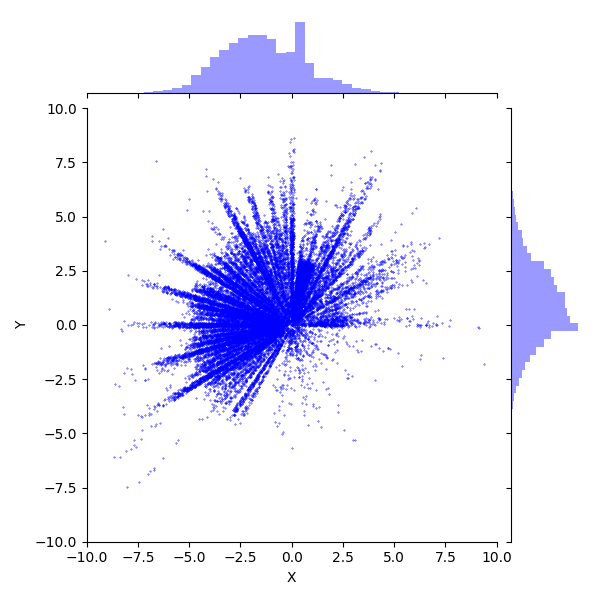
\includegraphics[width=0.95\textwidth]{../res_u_21/1/XYobj.png}
\end{minipage}
\hfill
\begin{minipage}[h]{0.49\linewidth}
        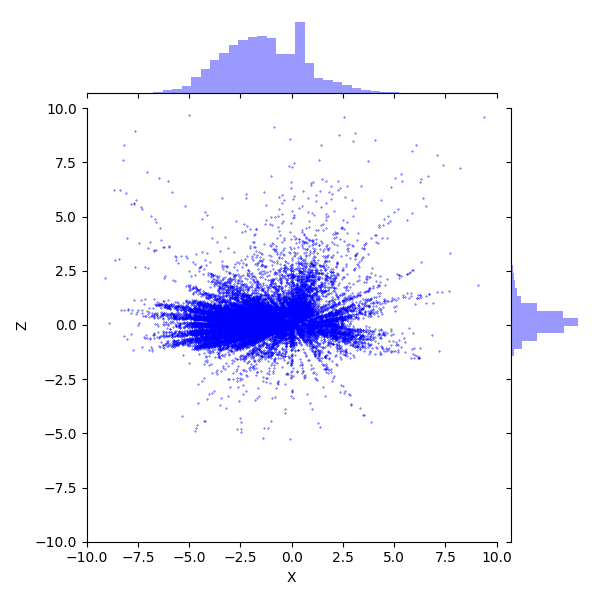
\includegraphics[width=0.95\textwidth]{../res_u_21/1/XZobj.png}
\end{minipage}
\end{figure}


\pagebreak

\begin{figure}[h!]
\caption{Распределение объектов в галактических координатах.}
\begin{minipage}[h]{0.49\linewidth}
        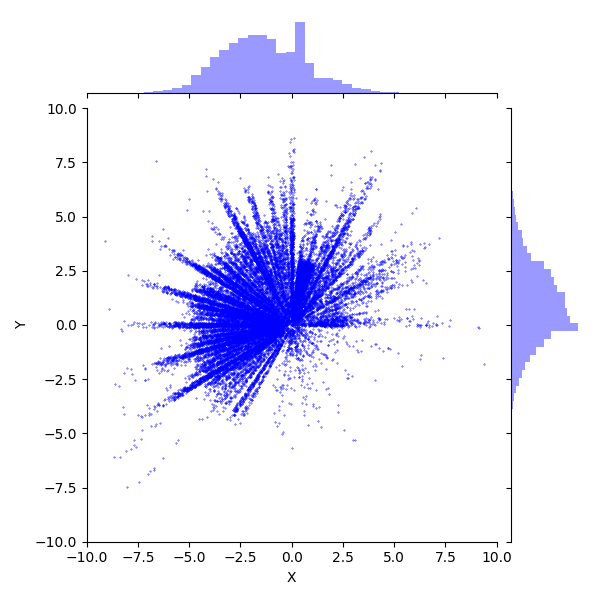
\includegraphics[width=0.95\textwidth]{../res_u_21/1/XYobj.png}
\end{minipage}
\hfill
\begin{minipage}[h]{0.49\linewidth}
        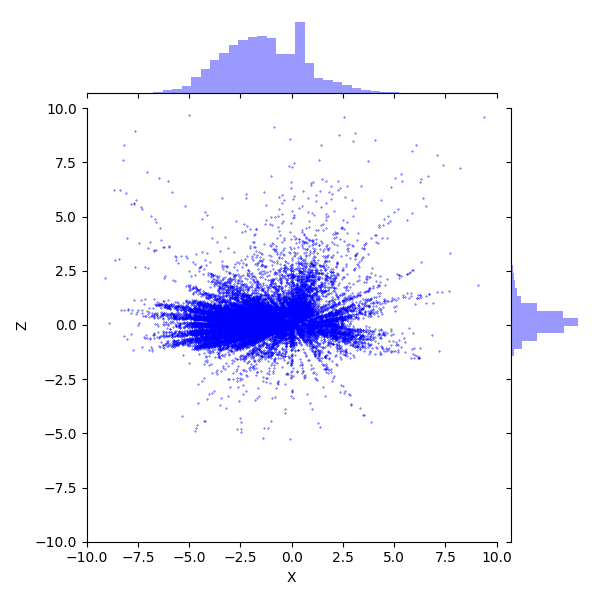
\includegraphics[width=0.95\textwidth]{../res_u_21/1/XZobj.png}
\end{minipage}
\end{figure}



\subsubsection*{Распределение ошибок скоростей:}
\begin{figure}[h!]
\caption{Распределение лучевых скоростей и их измертельных ошибок.}
\begin{minipage}[h]{0.49\linewidth}
        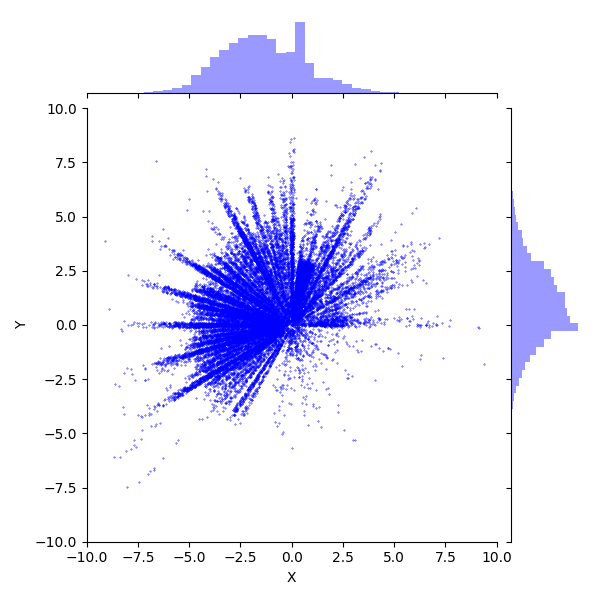
\includegraphics[width=0.95\textwidth]{../res_u_21/1/XYobj.png}
\end{minipage}
\hfill
\begin{minipage}[h]{0.49\linewidth}
        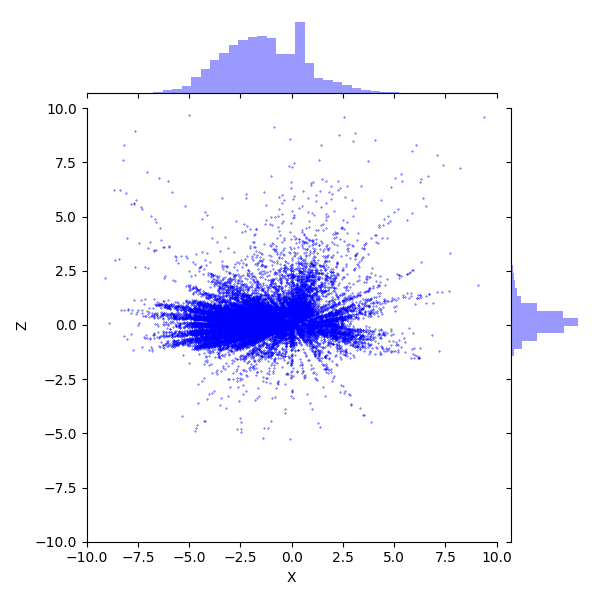
\includegraphics[width=0.95\textwidth]{../res_u_21/1/XZobj.png}
\end{minipage}
\end{figure}

\begin{figure}[h!]
\caption{Распределение ошибок собственных движений в каталоге UCAC-4.}
\begin{minipage}[h]{0.49\linewidth}
        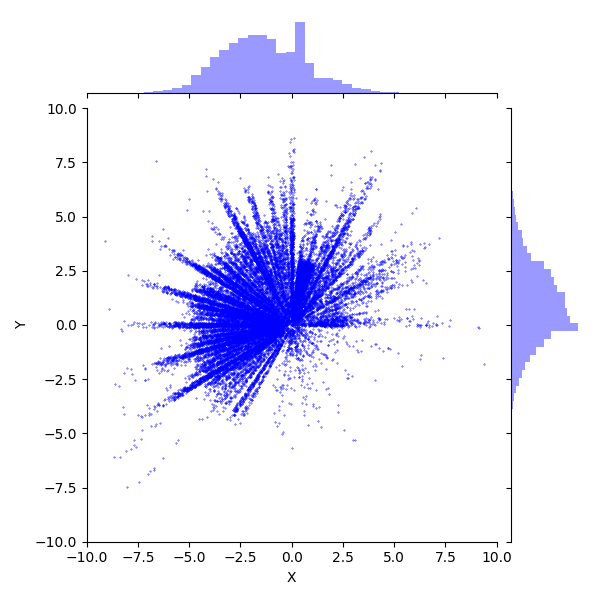
\includegraphics[width=0.95\textwidth]{../res_u_21/1/XYobj.png}
\end{minipage}
\hfill
\begin{minipage}[h]{0.49\linewidth}
        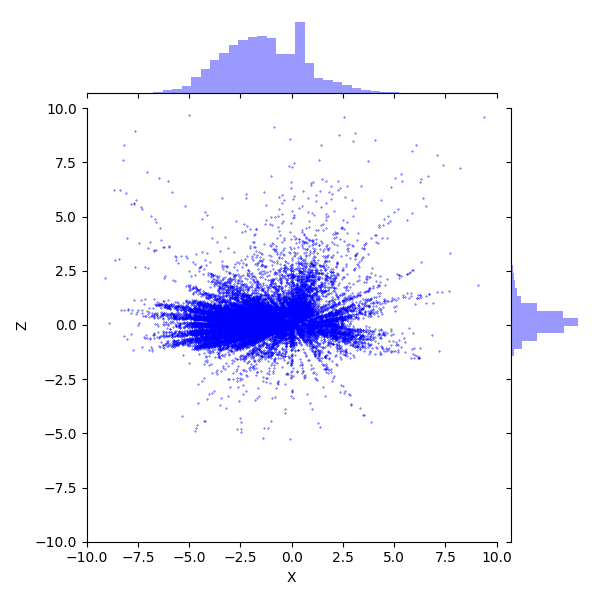
\includegraphics[width=0.95\textwidth]{../res_u_21/1/XZobj.png}
\end{minipage}
\end{figure}

\begin{figure}[h!]
\caption{Распределение ошибок собственных движений в каталоге HSOY.}
\begin{minipage}[h]{0.49\linewidth}
        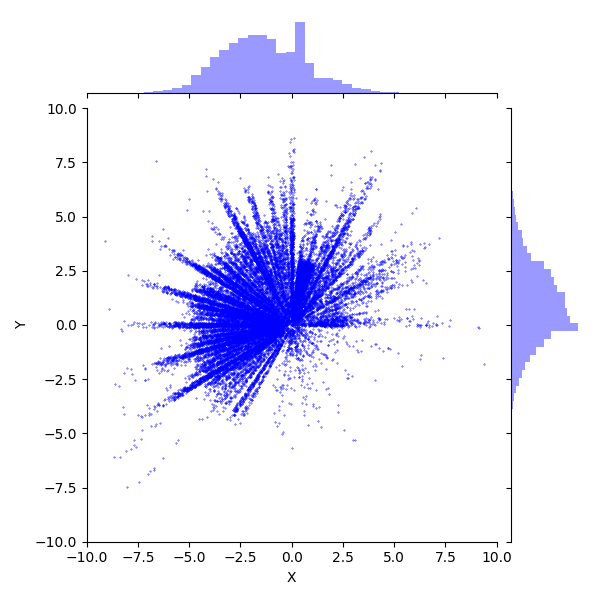
\includegraphics[width=0.95\textwidth]{../res_u_21/1/XYobj.png}
\end{minipage}
\hfill
\begin{minipage}[h]{0.49\linewidth}
        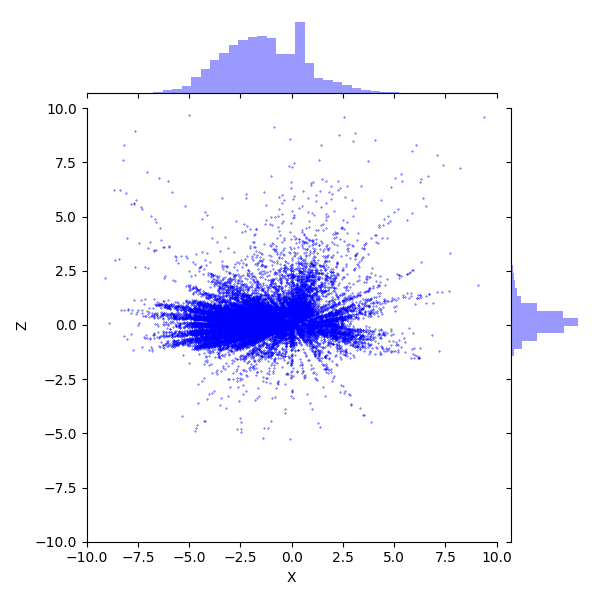
\includegraphics[width=0.95\textwidth]{../res_u_21/1/XZobj.png}
\end{minipage}
\end{figure}

\pagebreak
\subsubsection{Переход к галактической СК}
\par \paragraph{Собственные движения.} 
Так как в каталогах UCAC-4 и HSOY указаны данные о собственных движениях в экваториальной СК, нужно было осуществить преобразование $(\mu_{\alpha}, \mu_{\delta}) \rightarrow (\mu_l, \mu_b)$.
\begin{equation}
        \sin{b} = \sin{\delta} \cos(90^{\circ} - \delta_p) - \cos{\delta} \sin(\alpha - \alpha_p - 90^{\circ}) \sin(90^{\circ} - \delta_p),
\end{equation}
\begin{equation}
        \sin{\varphi} = \frac{\cos{\delta} \sin(\alpha - \alpha_p - 90^{\circ}) \cos(90^{\circ} - \delta_p) + \sin{\delta} \sin(90^{\circ} - \delta_p)}{\cos{b}},
\end{equation}
\begin{equation}
        \cos{\varphi} = \frac{ \cos{\delta} \cos(\alpha - \alpha_p - 90^{\circ})}{\cos{b}},
\end{equation}
\begin{equation}
        l = \varphi + \theta_p,
\end{equation}
где $\theta_p = 32.93192^{\circ}$, $\alpha_p = 192.85948^{\circ}$, $\delta_p = 27.12825^{\circ}$. Переход к собственным движениям в галактической СК:
\begin{equation}
        \mu_l = l(\alpha + \mu_{\alpha}, \delta + \mu_{\delta}) - l(\alpha, \delta),
\end{equation}
\begin{equation}
        \mu_b = b(\alpha + \mu_{\alpha}, \delta + \mu_{\delta}) - b(\alpha, \delta).
\end{equation}
Также необходимо подставлять в (\ref{l_sys}) $\mu_l^* = \mu_l \cos{b}$.

\par \paragraph{Ошибки собственных движений.} 
\par Так как в каталогах UCAC-4 и HSOY указаны ошибки собственных движений в экваториальных координатах, необходимо также привести их к галактической СК. Для этого используется формула распространения ошибок \cite{6}:
\begin{equation}
        \sigma_{\mu_l} = \sqrt{\left(\frac{\partial \mu_l}{\partial \alpha} \sigma_{\mu_{\alpha}} \right)^2 + \left(\frac{\partial \mu_l}{\partial\delta} \sigma_{\mu_{\delta}} \right)^2},
\end{equation}

\begin{equation}
        \sigma_{\mu_b} = \sqrt{\left(\frac{\partial \mu_b}{\partial \alpha} \sigma_{\mu_{\alpha}} \right)^2 + \left(\frac{\partial \mu_b}{\partial\delta} \sigma_{\mu_{\delta}} \right)^2}.
\end{equation}


\begin{table}[h!]
\centering
\caption{Наблюдательные данные (приведены на эпоху \texttt{J2000})}
\begin{tabular}{|l|l|l|}
\hline
\textbf{Величина} & \textbf{Обозначение} & \textbf{Ед. изм.} \\
\hline
Прямое восхождение & $\alpha$ & deg \\
Склонение & $\delta$ & deg \\
Галактическая долгота & $l$ & deg \\
Галактическая широта & $b$ & deg \\
\hline
Гелиоцентрическая лучевая скорость & $V_{r, \mathrm{obs}}$ & km/s \\
Ошибка лучевой скорости & $\sigma_{V_{r, i}}$ & km/s \\
Гелиоцентрическое расстояние & $r$ & kpc \\
\hline
Проекция собственного движения по $\alpha$  & $\mu_{\alpha}* \cos{\delta}$ & mas/yr \\
Собственное движение по $\delta$  & $\mu_{\delta}$ & mas/yr \\
Ошибка собственного движения по $\alpha$  & $\sigma_{\mu_{\alpha}, i}$ & mas/yr \\
Ошибка собственного движения по $\delta$  & $\sigma_{\mu_{\delta}, i}$ & mas/yr \\
\hline
\end{tabular}
\end{table}


\subsubsection{Формирование выборок для оценки ошибок параметров методом \\ Монте-Карло} \label{mk}
Несмотря на то, что при частном решении используется обычный МНК, получать из матрицы ковариаций ошибки параметров некорректно, так как производится оптимизация по нелинейному параметру. Для того, чтобы исключить смещение и обеспечить состоятельность и эффектривность оценки ошибков параметров модели, используется метод Монте-Карло. Для получения ошибок параметров при решении (\ref{v_r_sys}) - (\ref{l_sys}), а также (\ref{chi_sq_func}), формируются псевдослучайные каталоги. В каждом из них такие же сведения о $l$, $b$, $r$, как в оригинальном APOGEE-RC ($\alpha$ и $\delta$ для решения систем не нужны). Лучевые скорости и собственные движения получались как
\begin{equation}
        V_{r, i}^{*} \in \mathcal{N} \left[ V_{r, \mathrm{mod}}(l_i, b_i, r_i),\sigma^2_{V_r} \right],
\end{equation}
\begin{equation}
        \mu_{b, i}^{*} \in \mathcal{N} \left[ \mu_{b, \mathrm{mod}}(l_i, b_i, r_i),\sigma^2_{\mu_b} \right],
\end{equation}
\begin{equation}
        \mu_{l, i}^{*} \in \mathcal{N} \left[ \mu_{l, \mathrm{mod}}(l_i, b_i, r_i),\sigma^2_{\mu_l} \right].
\end{equation}
\par После этого для каждого каталога находятся все параметры модели и строится кривая вращения. По совокупности всех найденных значений производится окончательная оценка параметров и построение доверительных областей кривой вращения.
\pagebreak
\subsection{Моделирование по лучевым скоростям}
Решается (\ref{v_r_sys}) с полным набором параметров. Порядок разложения $n < 10$. Итеративно применяется \ref{err_filter}, пока в выборке не будет объектов, попадающих под критерий (\ref{criteria}). После этого производится оценка ошибок параметров с помощью \ref{mk} по финальной выборке размера $N_{\mathrm{end}}$. Результаты приведены в таблице. 
\begin{table}[h!!]
\centering
\caption{Результаты.}
\begin{tabular}{r|rrrrrrrrrr}
\hline
$n$ & $1$ & $2$ & $3$ & $\textbf{4}$ & $5$&$ 6 $&$ 7 $&$ 8 $&$ 9 $&$ 10 $\\\hline
$N_{\mathrm{end}}$ & $1$ & $2$ & $3$ & $\textbf{4}$ & $5$&$ 6 $&$ 7 $&$ 8 $&$ 9 $&$ 10 $\\\hline
 $R_0 $&$     8.73$&$    8.73$&$    8.20$&$   \textbf{ 8.25}$&$    8.20$&$    8.18$&$    8.26$&$    8.27$&$    8.37$&$    8.54$\\$
 \sigma_{R_0} $&$     0.26$&$    0.32$&$   0.26$&$  \textbf{  0.25}$&$    0.25$&$    0.26$&$    0.28$&$    0.28$&$    0.30$&$    0.31$\\$
 \sigma_{V_r} $&$    30.50$&$   30.50$&$   30.36$&$  \textbf{ 30.36}$&$   30.35$&$   30.35$&$   30.35$&$   30.35$&$   30.34$&$   30.33$\\\hline$
 u_{\odot} $&$    13.19$&$   13.19$&$   13.56$&$  \textbf{ 13.61}$&$   13.61$&$   13.62$&$   13.60$&$   13.60$&$   13.58$&$   13.57$\\$
 \sigma_{u_{\odot}} $&$     0.30$&$    0.31$&$    0.31$&$   \textbf{ 0.31}$&$    0.31$&$    0.31$&$    0.31$&$    0.31$&$    0.31$&$    0.31$\\\hline$
 v_{\odot} $&$    27.12$&$   27.11$&$   24.92$&$  \textbf{ 25.41}$&$   25.00$&$   25.02$&$   24.77$&$   24.69$&$   24.25$&$   24.45$\\$
 \sigma_{v_{\odot}}$&$     0.41$&$    0.45$&$    0.46$&$   \textbf{ 0.48}$&$    0.50$&$    0.51$&$    0.53$&$    0.53$&$    0.56$&$    0.56$\\\hline$
 w_{\odot} $&$     3.96$&$    3.96$&$    4.70$&$   \textbf{ 4.71}$&$    4.85$&$    4.86$&$    4.93$&$    4.88$&$    4.97$&$    5.00$\\$
 \sigma_{w_{\odot}} $&$     0.84$&$    0.84$&$    0.84$&$   \textbf{ 0.84}$&$    0.84$&$    0.84$&$    0.84$&$    0.84$&$    0.84$&$    0.84$\\\hline$
 A $&$    13.44$&$   13.44$&$   15.35$&$  \textbf{ 15.85}$&$   16.05$&$   16.15$&$   16.23$&$   15.77$&$   15.66$&$   16.08$\\$
 \sigma(A) $&$     0.13$&$    0.15$&$    0.20$&$   \textbf{ 0.25}$&$    0.26$&$    0.31$&$    0.32$&$    0.39$&$    0.39$&$    0.45$\\$
 \theta_2$&$ $-$ $&$   -0.00$&$   -1.64$&$   \textbf{-0.62}$&$   -1.49$&$   -1.37$&$   -2.61$&$   -2.94$&$   -5.66$&$   -5.80$\\$
 \sigma(\theta_2)$&$ $-$ $&$    0.18$&$    0.21$&$  \textbf{  0.35}$&$    0.50$&$    0.56$&$    0.79$&$    0.81$&$    1.13$&$    1.13$\\$
 \theta_3$&$ $-$ $&$ $-$ $&$    2.35$&$   \textbf{ 3.03}$&$    3.77$&$    4.04$&$    4.87$&$    2.54$&$    2.78$&$    6.41$\\$
 \sigma(\theta_3)$&$ $-$ $&$ $-$ $&$    0.18$&$   \textbf{ 0.26}$&$    0.40$&$    0.66$&$    0.77$&$    1.37$&$    1.37$&$    2.16$\\$
 \theta_4$&$ $-$ $&$ $-$ $&$ $-$ $&$  \textbf{ -0.78}$&$   -0.10$&$   -0.33$&$    1.71$&$    3.06$&$   10.59$&$   10.43$\\$
 \sigma(\theta_4)$&$ $-$ $&$ $-$ $&$ $-$ $&$   \textbf{ 0.22}$&$    0.36$&$    0.58$&$    1.06$&$    1.24$&$    2.48$&$    2.51$\\$
 \theta_5$&$ $-$ $&$ $-$ $&$ $-$ $&$ $-$ $&$   -0.70$&$   -0.92$&$   -2.64$&$    1.21$&$   -1.79$&$  -12.10$\\$
 \sigma(\theta_5)$&$ $-$ $&$ $-$ $&$ $-$ $&$ $-$ $&$    0.29$&$    0.52$&$    0.93$&$    2.09$&$    2.27$&$    5.07$\\$
 \theta_6$&$ $-$ $&$ $-$ $&$ $-$ $&$ $-$ $&$ $-$ $&$    0.23$&$   -1.48$&$   -4.59$&$  -18.41$&$  -14.87$\\$
 \sigma(\theta_6)$&$ $-$ $&$ $-$ $&$ $-$ $&$ $-$ $&$ $-$ $&$    0.45$&$    0.86$&$    1.74$&$    4.31$&$    4.72$\\$
 \theta_7$&$ $-$ $&$ $-$ $&$ $-$ $&$ $-$ $&$ $-$ $&$ $-$ $&$    1.80$&$   -1.49$&$    8.18$&$   28.37$\\$
 \sigma(\theta_7)$&$ $-$ $&$ $-$ $&$ $-$ $&$ $-$ $&$ $-$ $&$ $-$ $&$    0.79$&$    1.79$&$    3.30$&$    9.36$\\$
 \theta_8$&$ $-$ $&$ $-$ $&$ $-$ $&$ $-$ $&$ $-$ $&$ $-$ $&$ $-$ $&$    3.46$&$   16.45$&$    3.05$\\$
 \sigma(\theta_8)$&$ $-$ $&$ $-$ $&$ $-$ $&$ $-$ $&$ $-$ $&$ $-$ $&$ $-$ $&$    1.69$&$    4.09$&$    7.38$\\$
 \theta_9$&$ $-$ $&$ $-$ $&$ $-$ $&$ $-$ $&$ $-$ $&$ $-$ $&$ $-$ $&$ $-$ $&$  -12.98$&$  -33.60$\\$
 \sigma(\theta_9)$&$ $-$ $&$ $-$ $&$ $-$ $&$ $-$ $&$ $-$ $&$ $-$ $&$ $-$ $&$ $-$ $&$    3.73$&$    9.64$\\$
 \theta_{10}$&$ $-$ $&$ $-$ $&$ $-$ $&$ $-$ $&$ $-$ $&$ $-$ $&$ $-$ $&$ $-$ $&$ $-$ $&$   20.41$\\$
 \sigma(\theta_{10})$&$ $-$ $&$ $-$ $&$ $-$ $&$ $-$ $&$ $-$ $&$ $-$ $&$ $-$ $&$ $-$ $&$ $-$ $&$    8.94$\\
\end{tabular}
\end{table}

\pagebreak
\paragraph{Кривая вращения.} Приводятся кривые вращения, полученные для различных $n$. При построении полагали значение $\omega_{\odot} = 30.5$ км/c/кпк.
%\begin{figure}[h!]
%\begin{minipage}[h]{0.49\linewidth}
%        \includegraphics[width=0.9\textwidth]{result_1_500_apogee-ucac_1/apogee-ucac.txt_1.eps}
%\end{minipage}
%\hfill
%\begin{minipage}[h]{0.49\linewidth}
%        \includegraphics[width=0.9\textwidth]{result_1_500_apogee-ucac_1/apogee-ucac.txt_1.eps}
%\end{minipage}
%\end{figure}
%\begin{figure}[h!]
%\begin{minipage}[h]{0.49\linewidth}
%        \includegraphics[width=0.9\textwidth]{result_1_500_apogee-ucac_1/apogee-ucac.txt_1.eps}
%\end{minipage}
%\hfill
%\begin{minipage}[h]{0.49\linewidth}
%        \includegraphics[width=0.9\textwidth]{result_1_500_apogee-ucac_1/apogee-ucac.txt_1.eps}
%\end{minipage}
%\end{figure}
%\begin{figure}[h!]
%\begin{minipage}[h]{0.49\linewidth}
%        \includegraphics[width=0.9\textwidth]{result_1_500_apogee-ucac_1/apogee-ucac.txt_1.eps}
%\end{minipage}
%\hfill
%\begin{minipage}[h]{0.49\linewidth}
%        \includegraphics[width=0.9\textwidth]{result_1_500_apogee-ucac_1/apogee-ucac.txt_1.eps}
%\end{minipage}
%\end{figure}


\pagebreak
\subsection{Моделирование по собственным движениям}
Решается (\ref{l_sys}) с полным набором параметров. Порядок разложения $n < 10$. Итеративно применяется \ref{err_filter}, пока в выборке не будет объектов, попадающих под критерий (\ref{criteria}). После этого производится оценка ошибок параметров с помощью \ref{mk} по финальной выборке размера $N_{\mathrm{end}}$. Результаты приведены в таблице. 
\begin{table}[h!!]
\centering
\caption{Результаты.}
\begin{tabular}{r|rrrrrrrrrr}
\hline
$n$ & $1$ & $2$ & $3$ & $\textbf{4}$ & $5$&$ 6 $&$ 7 $&$ 8 $&$ 9 $&$ 10 $\\\hline
$N_{\mathrm{end}}$ & $1$ & $2$ & $3$ & $\textbf{4}$ & $5$&$ 6 $&$ 7 $&$ 8 $&$ 9 $&$ 10 $\\\hline$
 R_0 $&$     8.73$&$    8.73$&$    8.20$&$   \textbf{ 8.25}$&$    8.20$&$    8.18$&$    8.26$&$    8.27$&$    8.37$&$    8.54$\\$
 \sigma_{R_0} $&$     0.26$&$    0.32$&$   0.26$&$  \textbf{  0.25}$&$    0.25$&$    0.26$&$    0.28$&$    0.28$&$    0.30$&$    0.31$\\$
 \sigma_{\mu_l} $&$    30.50$&$   30.50$&$   30.36$&$  \textbf{ 30.36}$&$   30.35$&$   30.35$&$   30.35$&$   30.35$&$   30.34$&$   30.33$\\\hline$
 u_{\odot} $&$    13.19$&$   13.19$&$   13.56$&$  \textbf{ 13.61}$&$   13.61$&$   13.62$&$   13.60$&$   13.60$&$   13.58$&$   13.57$\\$
 \sigma_{u_{\odot}} $&$     0.30$&$    0.31$&$    0.31$&$   \textbf{ 0.31}$&$    0.31$&$    0.31$&$    0.31$&$    0.31$&$    0.31$&$    0.31$\\\hline$
 v_{\odot} $&$    27.12$&$   27.11$&$   24.92$&$  \textbf{ 25.41}$&$   25.00$&$   25.02$&$   24.77$&$   24.69$&$   24.25$&$   24.45$\\$
 \sigma_{v_{\odot}}$&$     0.41$&$    0.45$&$    0.46$&$   \textbf{ 0.48}$&$    0.50$&$    0.51$&$    0.53$&$    0.53$&$    0.56$&$    0.56$\\\hline$
 \omega_0 $&$     3.96$&$    3.96$&$    4.70$&$   \textbf{ 4.71}$&$    4.85$&$    4.86$&$    4.93$&$    4.88$&$    4.97$&$    5.00$\\$
 \sigma_{\omega_0} $&$     0.84$&$    0.84$&$    0.84$&$   \textbf{ 0.84}$&$    0.84$&$    0.84$&$    0.84$&$    0.84$&$    0.84$&$    0.84$\\\hline$
 A $&$    13.44$&$   13.44$&$   15.35$&$  \textbf{ 15.85}$&$   16.05$&$   16.15$&$   16.23$&$   15.77$&$   15.66$&$   16.08$\\$
 \sigma(A) $&$     0.13$&$    0.15$&$    0.20$&$   \textbf{ 0.25}$&$    0.26$&$    0.31$&$    0.32$&$    0.39$&$    0.39$&$    0.45$\\$
 \theta_2$&$ $-$ $&$   -0.00$&$   -1.64$&$   \textbf{-0.62}$&$   -1.49$&$   -1.37$&$   -2.61$&$   -2.94$&$   -5.66$&$   -5.80$\\$
 \sigma(\theta_2)$&$ $-$ $&$    0.18$&$    0.21$&$  \textbf{  0.35}$&$    0.50$&$    0.56$&$    0.79$&$    0.81$&$    1.13$&$    1.13$\\$
 \theta_3$&$ $-$ $&$ $-$ $&$    2.35$&$   \textbf{ 3.03}$&$    3.77$&$    4.04$&$    4.87$&$    2.54$&$    2.78$&$    6.41$\\$
 \sigma(\theta_3)$&$ $-$ $&$ $-$ $&$    0.18$&$   \textbf{ 0.26}$&$    0.40$&$    0.66$&$    0.77$&$    1.37$&$    1.37$&$    2.16$\\$
 \theta_4$&$ $-$ $&$ $-$ $&$ $-$ $&$  \textbf{ -0.78}$&$   -0.10$&$   -0.33$&$    1.71$&$    3.06$&$   10.59$&$   10.43$\\$
 \sigma(\theta_4)$&$ $-$ $&$ $-$ $&$ $-$ $&$   \textbf{ 0.22}$&$    0.36$&$    0.58$&$    1.06$&$    1.24$&$    2.48$&$    2.51$\\$
 \theta_5$&$ $-$ $&$ $-$ $&$ $-$ $&$ $-$ $&$   -0.70$&$   -0.92$&$   -2.64$&$    1.21$&$   -1.79$&$  -12.10$\\$
 \sigma(\theta_5)$&$ $-$ $&$ $-$ $&$ $-$ $&$ $-$ $&$    0.29$&$    0.52$&$    0.93$&$    2.09$&$    2.27$&$    5.07$\\$
 \theta_6$&$ $-$ $&$ $-$ $&$ $-$ $&$ $-$ $&$ $-$ $&$    0.23$&$   -1.48$&$   -4.59$&$  -18.41$&$  -14.87$\\$
 \sigma(\theta_6)$&$ $-$ $&$ $-$ $&$ $-$ $&$ $-$ $&$ $-$ $&$    0.45$&$    0.86$&$    1.74$&$    4.31$&$    4.72$\\$
 \theta_7$&$ $-$ $&$ $-$ $&$ $-$ $&$ $-$ $&$ $-$ $&$ $-$ $&$    1.80$&$   -1.49$&$    8.18$&$   28.37$\\$
 \sigma(\theta_7)$&$ $-$ $&$ $-$ $&$ $-$ $&$ $-$ $&$ $-$ $&$ $-$ $&$    0.79$&$    1.79$&$    3.30$&$    9.36$\\$
 \theta_8$&$ $-$ $&$ $-$ $&$ $-$ $&$ $-$ $&$ $-$ $&$ $-$ $&$ $-$ $&$    3.46$&$   16.45$&$    3.05$\\$
 \sigma(\theta_8)$&$ $-$ $&$ $-$ $&$ $-$ $&$ $-$ $&$ $-$ $&$ $-$ $&$ $-$ $&$    1.69$&$    4.09$&$    7.38$\\$
 \theta_9$&$ $-$ $&$ $-$ $&$ $-$ $&$ $-$ $&$ $-$ $&$ $-$ $&$ $-$ $&$ $-$ $&$  -12.98$&$  -33.60$\\$
 \sigma(\theta_9)$&$ $-$ $&$ $-$ $&$ $-$ $&$ $-$ $&$ $-$ $&$ $-$ $&$ $-$ $&$ $-$ $&$    3.73$&$    9.64$\\$
 \theta_{10}$&$ $-$ $&$ $-$ $&$ $-$ $&$ $-$ $&$ $-$ $&$ $-$ $&$ $-$ $&$ $-$ $&$ $-$ $&$   20.41$\\$
 \sigma(\theta_{10})$&$ $-$ $&$ $-$ $&$ $-$ $&$ $-$ $&$ $-$ $&$ $-$ $&$ $-$ $&$ $-$ $&$ $-$ $&$    8.94$\\
\end{tabular}
\end{table}

Аналогичного отдельного решения для системы (\ref{b_sys}) получить не удалось, так как профиль целевой функции в этом случае не имеет минимума на разумных $R_0$. В целом система (\ref{b_sys}) нужна для уточнения компоненты $w_{\odot}$ остаточного движения Солнца при уже заданном $R_0$.
\pagebreak
\paragraph{Кривая вращения.} Приводятся кривые вращения, полученные для различных $n$. 

        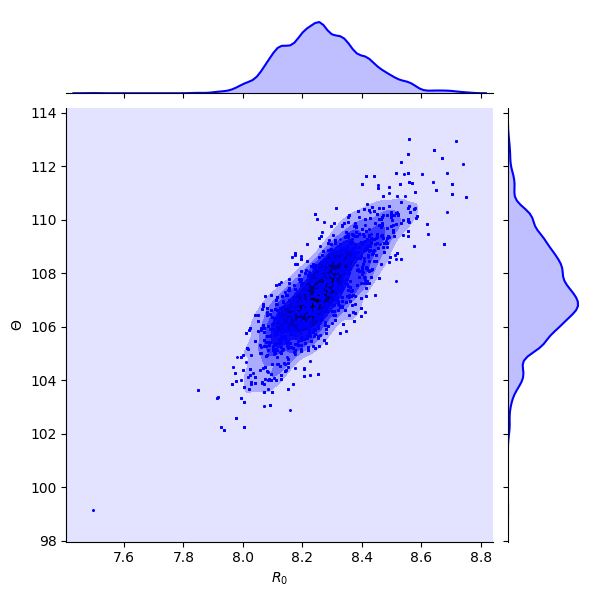
\includegraphics[width=0.9\textwidth]{../../sources/scripts/out.png}
\pagebreak
\subsection{Трехкомпонентное моделирование}
\subsubsection{Результаты по уравнению без природной дисперсии}
Вариант решения \ref{united_mod}. Порядок разложения $n < 10$. Итеративно применяется \ref{err_filter} для всех компонент -- модельных лучевых скоростей и собственных движений. После этого производится оценка ошибок параметров с помощью \ref{mk} по финальной выборке размера $N_{\mathrm{end}}$. Результаты приведены в таблице. 
\begin{table}[h!!]
\centering
\caption{APOGEE-RC с собственными движениями UCAC-4.}
\begin{tabular}{r|rrrrrrrrrr}
\hline
$n$ & $1$ & $2$ & $3$ & $\textbf{4}$ & $5$&$ 6 $&$ 7 $&$ 8 $&$ 9 $&$ 10 $\\\hline
$N_{\mathrm{end}}$ & $1$ & $2$ & $3$ & $\textbf{4}$ & $5$&$ 6 $&$ 7 $&$ 8 $&$ 9 $&$ 10 $\\\hline$
 R_0 $&$     8.73$&$    8.73$&$    8.20$&$   \textbf{ 8.25}$&$    8.20$&$    8.18$&$    8.26$&$    8.27$&$    8.37$&$    8.54$\\$
 \sigma_{R_0} $&$     0.26$&$    0.32$&$   0.26$&$  \textbf{  0.25}$&$    0.25$&$    0.26$&$    0.28$&$    0.28$&$    0.30$&$    0.31$\\$
 \sigma_{\mu_l} $&$    30.50$&$   30.50$&$   30.36$&$  \textbf{ 30.36}$&$   30.35$&$   30.35$&$   30.35$&$   30.35$&$   30.34$&$   30.33$\\\hline$
 u_{\odot} $&$    13.19$&$   13.19$&$   13.56$&$  \textbf{ 13.61}$&$   13.61$&$   13.62$&$   13.60$&$   13.60$&$   13.58$&$   13.57$\\$
 \sigma_{u_{\odot}} $&$     0.30$&$    0.31$&$    0.31$&$   \textbf{ 0.31}$&$    0.31$&$    0.31$&$    0.31$&$    0.31$&$    0.31$&$    0.31$\\\hline$
 v_{\odot} $&$    27.12$&$   27.11$&$   24.92$&$  \textbf{ 25.41}$&$   25.00$&$   25.02$&$   24.77$&$   24.69$&$   24.25$&$   24.45$\\$
 \sigma_{v_{\odot}}$&$     0.41$&$    0.45$&$    0.46$&$   \textbf{ 0.48}$&$    0.50$&$    0.51$&$    0.53$&$    0.53$&$    0.56$&$    0.56$\\\hline$
 \omega_0 $&$     3.96$&$    3.96$&$    4.70$&$   \textbf{ 4.71}$&$    4.85$&$    4.86$&$    4.93$&$    4.88$&$    4.97$&$    5.00$\\$
 \sigma_{\omega_0} $&$     0.84$&$    0.84$&$    0.84$&$   \textbf{ 0.84}$&$    0.84$&$    0.84$&$    0.84$&$    0.84$&$    0.84$&$    0.84$\\\hline$
 A $&$    13.44$&$   13.44$&$   15.35$&$  \textbf{ 15.85}$&$   16.05$&$   16.15$&$   16.23$&$   15.77$&$   15.66$&$   16.08$\\$
 \sigma(A) $&$     0.13$&$    0.15$&$    0.20$&$   \textbf{ 0.25}$&$    0.26$&$    0.31$&$    0.32$&$    0.39$&$    0.39$&$    0.45$\\$
 \theta_2$&$ $-$ $&$   -0.00$&$   -1.64$&$   \textbf{-0.62}$&$   -1.49$&$   -1.37$&$   -2.61$&$   -2.94$&$   -5.66$&$   -5.80$\\$
 \sigma(\theta_2)$&$ $-$ $&$    0.18$&$    0.21$&$  \textbf{  0.35}$&$    0.50$&$    0.56$&$    0.79$&$    0.81$&$    1.13$&$    1.13$\\$
 \theta_3$&$ $-$ $&$ $-$ $&$    2.35$&$   \textbf{ 3.03}$&$    3.77$&$    4.04$&$    4.87$&$    2.54$&$    2.78$&$    6.41$\\$
 \sigma(\theta_3)$&$ $-$ $&$ $-$ $&$    0.18$&$   \textbf{ 0.26}$&$    0.40$&$    0.66$&$    0.77$&$    1.37$&$    1.37$&$    2.16$\\$
 \theta_4$&$ $-$ $&$ $-$ $&$ $-$ $&$  \textbf{ -0.78}$&$   -0.10$&$   -0.33$&$    1.71$&$    3.06$&$   10.59$&$   10.43$\\$
 \sigma(\theta_4)$&$ $-$ $&$ $-$ $&$ $-$ $&$   \textbf{ 0.22}$&$    0.36$&$    0.58$&$    1.06$&$    1.24$&$    2.48$&$    2.51$\\$
 \theta_5$&$ $-$ $&$ $-$ $&$ $-$ $&$ $-$ $&$   -0.70$&$   -0.92$&$   -2.64$&$    1.21$&$   -1.79$&$  -12.10$\\$
 \sigma(\theta_5)$&$ $-$ $&$ $-$ $&$ $-$ $&$ $-$ $&$    0.29$&$    0.52$&$    0.93$&$    2.09$&$    2.27$&$    5.07$\\$
 \theta_6$&$ $-$ $&$ $-$ $&$ $-$ $&$ $-$ $&$ $-$ $&$    0.23$&$   -1.48$&$   -4.59$&$  -18.41$&$  -14.87$\\$
 \sigma(\theta_6)$&$ $-$ $&$ $-$ $&$ $-$ $&$ $-$ $&$ $-$ $&$    0.45$&$    0.86$&$    1.74$&$    4.31$&$    4.72$\\$
 \theta_7$&$ $-$ $&$ $-$ $&$ $-$ $&$ $-$ $&$ $-$ $&$ $-$ $&$    1.80$&$   -1.49$&$    8.18$&$   28.37$\\$
 \sigma(\theta_7)$&$ $-$ $&$ $-$ $&$ $-$ $&$ $-$ $&$ $-$ $&$ $-$ $&$    0.79$&$    1.79$&$    3.30$&$    9.36$\\$
 \theta_8$&$ $-$ $&$ $-$ $&$ $-$ $&$ $-$ $&$ $-$ $&$ $-$ $&$ $-$ $&$    3.46$&$   16.45$&$    3.05$\\$
 \sigma(\theta_8)$&$ $-$ $&$ $-$ $&$ $-$ $&$ $-$ $&$ $-$ $&$ $-$ $&$ $-$ $&$    1.69$&$    4.09$&$    7.38$\\$
 \theta_9$&$ $-$ $&$ $-$ $&$ $-$ $&$ $-$ $&$ $-$ $&$ $-$ $&$ $-$ $&$ $-$ $&$  -12.98$&$  -33.60$\\$
 \sigma(\theta_9)$&$ $-$ $&$ $-$ $&$ $-$ $&$ $-$ $&$ $-$ $&$ $-$ $&$ $-$ $&$ $-$ $&$    3.73$&$    9.64$\\$
 \theta_{10}$&$ $-$ $&$ $-$ $&$ $-$ $&$ $-$ $&$ $-$ $&$ $-$ $&$ $-$ $&$ $-$ $&$ $-$ $&$   20.41$\\$
 \sigma(\theta_{10})$&$ $-$ $&$ $-$ $&$ $-$ $&$ $-$ $&$ $-$ $&$ $-$ $&$ $-$ $&$ $-$ $&$ $-$ $&$    8.94$\\
\end{tabular}
\end{table}


\pagebreak
\paragraph{Кривая вращения.} Приводятся кривые вращения, полученные для различных $n$. 

        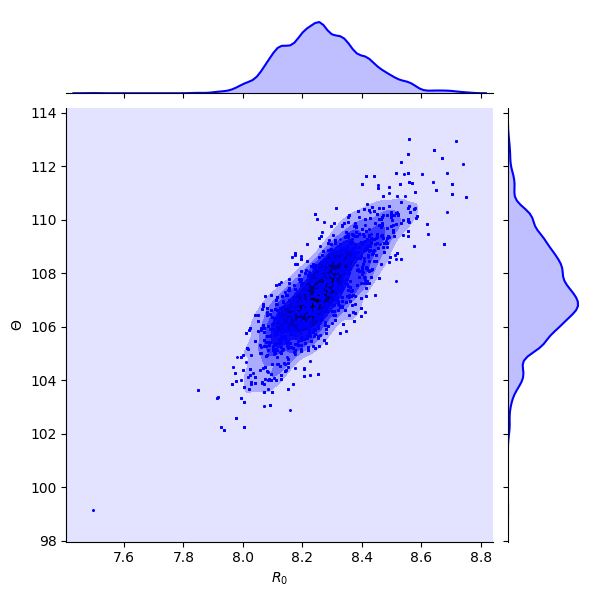
\includegraphics[width=0.9\textwidth]{../../sources/scripts/out.png}
\pagebreak

\begin{table}[h!!]
\centering
\caption{APOGEE-RC с собственными движениями HSOY.}
\begin{tabular}{r|rrrrrrrrrr}
\hline
$n$ & $1$ & $2$ & $3$ & $\textbf{4}$ & $5$&$ 6 $&$ 7 $&$ 8 $&$ 9 $&$ 10 $\\\hline
$N_{\mathrm{end}}$ & $1$ & $2$ & $3$ & $\textbf{4}$ & $5$&$ 6 $&$ 7 $&$ 8 $&$ 9 $&$ 10 $\\\hline$
 R_0 $&$     8.73$&$    8.73$&$    8.20$&$   \textbf{ 8.25}$&$    8.20$&$    8.18$&$    8.26$&$    8.27$&$    8.37$&$    8.54$\\$
 \sigma_{R_0} $&$     0.26$&$    0.32$&$   0.26$&$  \textbf{  0.25}$&$    0.25$&$    0.26$&$    0.28$&$    0.28$&$    0.30$&$    0.31$\\$
 \sigma_{\mu_l} $&$    30.50$&$   30.50$&$   30.36$&$  \textbf{ 30.36}$&$   30.35$&$   30.35$&$   30.35$&$   30.35$&$   30.34$&$   30.33$\\\hline$
 u_{\odot} $&$    13.19$&$   13.19$&$   13.56$&$  \textbf{ 13.61}$&$   13.61$&$   13.62$&$   13.60$&$   13.60$&$   13.58$&$   13.57$\\$
 \sigma_{u_{\odot}} $&$     0.30$&$    0.31$&$    0.31$&$   \textbf{ 0.31}$&$    0.31$&$    0.31$&$    0.31$&$    0.31$&$    0.31$&$    0.31$\\\hline$
 v_{\odot} $&$    27.12$&$   27.11$&$   24.92$&$  \textbf{ 25.41}$&$   25.00$&$   25.02$&$   24.77$&$   24.69$&$   24.25$&$   24.45$\\$
 \sigma_{v_{\odot}}$&$     0.41$&$    0.45$&$    0.46$&$   \textbf{ 0.48}$&$    0.50$&$    0.51$&$    0.53$&$    0.53$&$    0.56$&$    0.56$\\\hline$
 \omega_0 $&$     3.96$&$    3.96$&$    4.70$&$   \textbf{ 4.71}$&$    4.85$&$    4.86$&$    4.93$&$    4.88$&$    4.97$&$    5.00$\\$
 \sigma_{\omega_0} $&$     0.84$&$    0.84$&$    0.84$&$   \textbf{ 0.84}$&$    0.84$&$    0.84$&$    0.84$&$    0.84$&$    0.84$&$    0.84$\\\hline$
 A $&$    13.44$&$   13.44$&$   15.35$&$  \textbf{ 15.85}$&$   16.05$&$   16.15$&$   16.23$&$   15.77$&$   15.66$&$   16.08$\\$
 \sigma(A) $&$     0.13$&$    0.15$&$    0.20$&$   \textbf{ 0.25}$&$    0.26$&$    0.31$&$    0.32$&$    0.39$&$    0.39$&$    0.45$\\$
 \theta_2$&$ $-$ $&$   -0.00$&$   -1.64$&$   \textbf{-0.62}$&$   -1.49$&$   -1.37$&$   -2.61$&$   -2.94$&$   -5.66$&$   -5.80$\\$
 \sigma(\theta_2)$&$ $-$ $&$    0.18$&$    0.21$&$  \textbf{  0.35}$&$    0.50$&$    0.56$&$    0.79$&$    0.81$&$    1.13$&$    1.13$\\$
 \theta_3$&$ $-$ $&$ $-$ $&$    2.35$&$   \textbf{ 3.03}$&$    3.77$&$    4.04$&$    4.87$&$    2.54$&$    2.78$&$    6.41$\\$
 \sigma(\theta_3)$&$ $-$ $&$ $-$ $&$    0.18$&$   \textbf{ 0.26}$&$    0.40$&$    0.66$&$    0.77$&$    1.37$&$    1.37$&$    2.16$\\$
 \theta_4$&$ $-$ $&$ $-$ $&$ $-$ $&$  \textbf{ -0.78}$&$   -0.10$&$   -0.33$&$    1.71$&$    3.06$&$   10.59$&$   10.43$\\$
 \sigma(\theta_4)$&$ $-$ $&$ $-$ $&$ $-$ $&$   \textbf{ 0.22}$&$    0.36$&$    0.58$&$    1.06$&$    1.24$&$    2.48$&$    2.51$\\$
 \theta_5$&$ $-$ $&$ $-$ $&$ $-$ $&$ $-$ $&$   -0.70$&$   -0.92$&$   -2.64$&$    1.21$&$   -1.79$&$  -12.10$\\$
 \sigma(\theta_5)$&$ $-$ $&$ $-$ $&$ $-$ $&$ $-$ $&$    0.29$&$    0.52$&$    0.93$&$    2.09$&$    2.27$&$    5.07$\\$
 \theta_6$&$ $-$ $&$ $-$ $&$ $-$ $&$ $-$ $&$ $-$ $&$    0.23$&$   -1.48$&$   -4.59$&$  -18.41$&$  -14.87$\\$
 \sigma(\theta_6)$&$ $-$ $&$ $-$ $&$ $-$ $&$ $-$ $&$ $-$ $&$    0.45$&$    0.86$&$    1.74$&$    4.31$&$    4.72$\\$
 \theta_7$&$ $-$ $&$ $-$ $&$ $-$ $&$ $-$ $&$ $-$ $&$ $-$ $&$    1.80$&$   -1.49$&$    8.18$&$   28.37$\\$
 \sigma(\theta_7)$&$ $-$ $&$ $-$ $&$ $-$ $&$ $-$ $&$ $-$ $&$ $-$ $&$    0.79$&$    1.79$&$    3.30$&$    9.36$\\$
 \theta_8$&$ $-$ $&$ $-$ $&$ $-$ $&$ $-$ $&$ $-$ $&$ $-$ $&$ $-$ $&$    3.46$&$   16.45$&$    3.05$\\$
 \sigma(\theta_8)$&$ $-$ $&$ $-$ $&$ $-$ $&$ $-$ $&$ $-$ $&$ $-$ $&$ $-$ $&$    1.69$&$    4.09$&$    7.38$\\$
 \theta_9$&$ $-$ $&$ $-$ $&$ $-$ $&$ $-$ $&$ $-$ $&$ $-$ $&$ $-$ $&$ $-$ $&$  -12.98$&$  -33.60$\\$
 \sigma(\theta_9)$&$ $-$ $&$ $-$ $&$ $-$ $&$ $-$ $&$ $-$ $&$ $-$ $&$ $-$ $&$ $-$ $&$    3.73$&$    9.64$\\$
 \theta_{10}$&$ $-$ $&$ $-$ $&$ $-$ $&$ $-$ $&$ $-$ $&$ $-$ $&$ $-$ $&$ $-$ $&$ $-$ $&$   20.41$\\$
 \sigma(\theta_{10})$&$ $-$ $&$ $-$ $&$ $-$ $&$ $-$ $&$ $-$ $&$ $-$ $&$ $-$ $&$ $-$ $&$ $-$ $&$    8.94$\\
\end{tabular}
\end{table}


\pagebreak
\paragraph{Кривая вращения.} Приводятся кривые вращения, полученные для различных $n$. 

        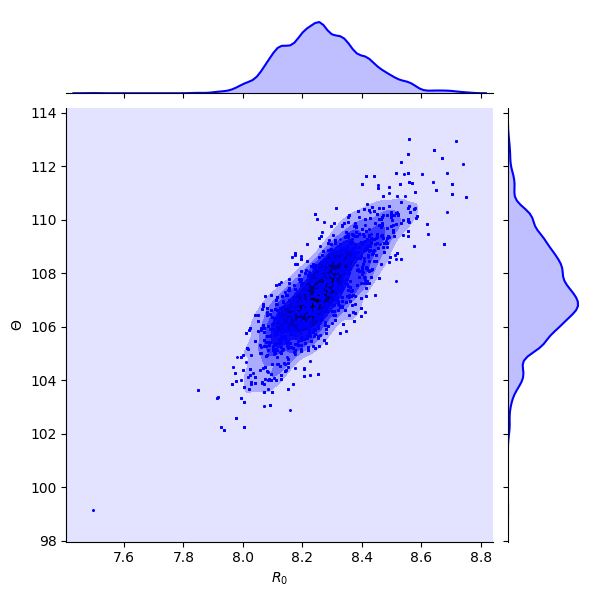
\includegraphics[width=0.9\textwidth]{../../sources/scripts/out.png}
\pagebreak

\subsubsection{Результаты по уравнению с природной дисперсией}
Вариант решения \ref{sigma_0_mode}. Порядок разложения $n < 10$. Итеративно применяется \ref{err_filter} для всех компонент -- модельных лучевых скоростей и собственных движений. После этого производится оценка ошибок параметров с помощью \ref{mk} по финальной выборке размера $N_{\mathrm{end}}$. Результаты приведены в таблице. 
\begin{table}[h!!]
\centering
\caption{APOGEE-RC с собственными движениями UCAC-4.}
\begin{tabular}{r|rrrrrrrrrr}
\hline
$n$ & $1$ & $2$ & $3$ & $\textbf{4}$ & $5$&$ 6 $&$ 7 $&$ 8 $&$ 9 $&$ 10 $\\\hline
$N_{\mathrm{end}}$ & $1$ & $2$ & $3$ & $\textbf{4}$ & $5$&$ 6 $&$ 7 $&$ 8 $&$ 9 $&$ 10 $\\\hline$
 R_0 $&$     8.73$&$    8.73$&$    8.20$&$   \textbf{ 8.25}$&$    8.20$&$    8.18$&$    8.26$&$    8.27$&$    8.37$&$    8.54$\\$
 \sigma_{R_0} $&$     0.26$&$    0.32$&$   0.26$&$  \textbf{  0.25}$&$    0.25$&$    0.26$&$    0.28$&$    0.28$&$    0.30$&$    0.31$\\$
 \sigma_{\mu_l} $&$    30.50$&$   30.50$&$   30.36$&$  \textbf{ 30.36}$&$   30.35$&$   30.35$&$   30.35$&$   30.35$&$   30.34$&$   30.33$\\\hline$
 u_{\odot} $&$    13.19$&$   13.19$&$   13.56$&$  \textbf{ 13.61}$&$   13.61$&$   13.62$&$   13.60$&$   13.60$&$   13.58$&$   13.57$\\$
 \sigma_{u_{\odot}} $&$     0.30$&$    0.31$&$    0.31$&$   \textbf{ 0.31}$&$    0.31$&$    0.31$&$    0.31$&$    0.31$&$    0.31$&$    0.31$\\\hline$
 v_{\odot} $&$    27.12$&$   27.11$&$   24.92$&$  \textbf{ 25.41}$&$   25.00$&$   25.02$&$   24.77$&$   24.69$&$   24.25$&$   24.45$\\$
 \sigma_{v_{\odot}}$&$     0.41$&$    0.45$&$    0.46$&$   \textbf{ 0.48}$&$    0.50$&$    0.51$&$    0.53$&$    0.53$&$    0.56$&$    0.56$\\\hline$
 \omega_0 $&$     3.96$&$    3.96$&$    4.70$&$   \textbf{ 4.71}$&$    4.85$&$    4.86$&$    4.93$&$    4.88$&$    4.97$&$    5.00$\\$
 \sigma_{\omega_0} $&$     0.84$&$    0.84$&$    0.84$&$   \textbf{ 0.84}$&$    0.84$&$    0.84$&$    0.84$&$    0.84$&$    0.84$&$    0.84$\\\hline$
 A $&$    13.44$&$   13.44$&$   15.35$&$  \textbf{ 15.85}$&$   16.05$&$   16.15$&$   16.23$&$   15.77$&$   15.66$&$   16.08$\\$
 \sigma(A) $&$     0.13$&$    0.15$&$    0.20$&$   \textbf{ 0.25}$&$    0.26$&$    0.31$&$    0.32$&$    0.39$&$    0.39$&$    0.45$\\$
 \theta_2$&$ $-$ $&$   -0.00$&$   -1.64$&$   \textbf{-0.62}$&$   -1.49$&$   -1.37$&$   -2.61$&$   -2.94$&$   -5.66$&$   -5.80$\\$
 \sigma(\theta_2)$&$ $-$ $&$    0.18$&$    0.21$&$  \textbf{  0.35}$&$    0.50$&$    0.56$&$    0.79$&$    0.81$&$    1.13$&$    1.13$\\$
 \theta_3$&$ $-$ $&$ $-$ $&$    2.35$&$   \textbf{ 3.03}$&$    3.77$&$    4.04$&$    4.87$&$    2.54$&$    2.78$&$    6.41$\\$
 \sigma(\theta_3)$&$ $-$ $&$ $-$ $&$    0.18$&$   \textbf{ 0.26}$&$    0.40$&$    0.66$&$    0.77$&$    1.37$&$    1.37$&$    2.16$\\$
 \theta_4$&$ $-$ $&$ $-$ $&$ $-$ $&$  \textbf{ -0.78}$&$   -0.10$&$   -0.33$&$    1.71$&$    3.06$&$   10.59$&$   10.43$\\$
 \sigma(\theta_4)$&$ $-$ $&$ $-$ $&$ $-$ $&$   \textbf{ 0.22}$&$    0.36$&$    0.58$&$    1.06$&$    1.24$&$    2.48$&$    2.51$\\$
 \theta_5$&$ $-$ $&$ $-$ $&$ $-$ $&$ $-$ $&$   -0.70$&$   -0.92$&$   -2.64$&$    1.21$&$   -1.79$&$  -12.10$\\$
 \sigma(\theta_5)$&$ $-$ $&$ $-$ $&$ $-$ $&$ $-$ $&$    0.29$&$    0.52$&$    0.93$&$    2.09$&$    2.27$&$    5.07$\\$
 \theta_6$&$ $-$ $&$ $-$ $&$ $-$ $&$ $-$ $&$ $-$ $&$    0.23$&$   -1.48$&$   -4.59$&$  -18.41$&$  -14.87$\\$
 \sigma(\theta_6)$&$ $-$ $&$ $-$ $&$ $-$ $&$ $-$ $&$ $-$ $&$    0.45$&$    0.86$&$    1.74$&$    4.31$&$    4.72$\\$
 \theta_7$&$ $-$ $&$ $-$ $&$ $-$ $&$ $-$ $&$ $-$ $&$ $-$ $&$    1.80$&$   -1.49$&$    8.18$&$   28.37$\\$
 \sigma(\theta_7)$&$ $-$ $&$ $-$ $&$ $-$ $&$ $-$ $&$ $-$ $&$ $-$ $&$    0.79$&$    1.79$&$    3.30$&$    9.36$\\$
 \theta_8$&$ $-$ $&$ $-$ $&$ $-$ $&$ $-$ $&$ $-$ $&$ $-$ $&$ $-$ $&$    3.46$&$   16.45$&$    3.05$\\$
 \sigma(\theta_8)$&$ $-$ $&$ $-$ $&$ $-$ $&$ $-$ $&$ $-$ $&$ $-$ $&$ $-$ $&$    1.69$&$    4.09$&$    7.38$\\$
 \theta_9$&$ $-$ $&$ $-$ $&$ $-$ $&$ $-$ $&$ $-$ $&$ $-$ $&$ $-$ $&$ $-$ $&$  -12.98$&$  -33.60$\\$
 \sigma(\theta_9)$&$ $-$ $&$ $-$ $&$ $-$ $&$ $-$ $&$ $-$ $&$ $-$ $&$ $-$ $&$ $-$ $&$    3.73$&$    9.64$\\$
 \theta_{10}$&$ $-$ $&$ $-$ $&$ $-$ $&$ $-$ $&$ $-$ $&$ $-$ $&$ $-$ $&$ $-$ $&$ $-$ $&$   20.41$\\$
 \sigma(\theta_{10})$&$ $-$ $&$ $-$ $&$ $-$ $&$ $-$ $&$ $-$ $&$ $-$ $&$ $-$ $&$ $-$ $&$ $-$ $&$    8.94$\\
\end{tabular}
\end{table}


\pagebreak
\paragraph{Кривая вращения.} Приводятся кривые вращения, полученные для различных $n$. 

        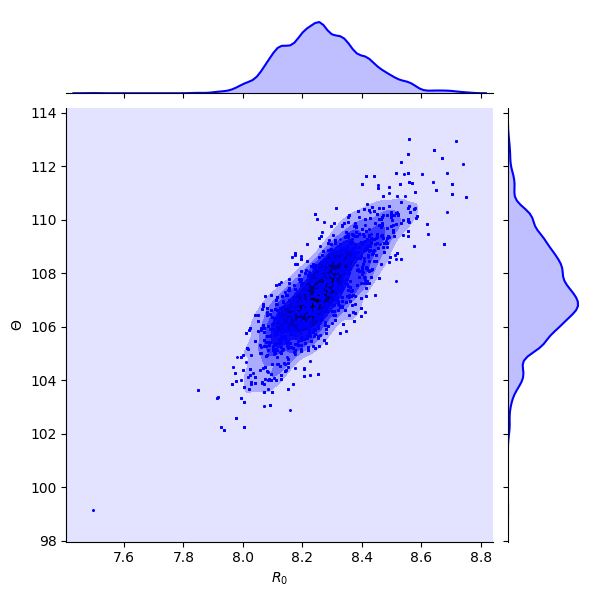
\includegraphics[width=0.9\textwidth]{../../sources/scripts/out.png}
\pagebreak
\begin{table}[h!!]
\centering
\caption{APOGEE-RC с собственными движениями HSOY.}
\begin{tabular}{r|rrrrrrrrrr}
\hline
$n$ & $1$ & $2$ & $3$ & $\textbf{4}$ & $5$&$ 6 $&$ 7 $&$ 8 $&$ 9 $&$ 10 $\\\hline
$N_{\mathrm{end}}$ & $1$ & $2$ & $3$ & $\textbf{4}$ & $5$&$ 6 $&$ 7 $&$ 8 $&$ 9 $&$ 10 $\\\hline$
 R_0 $&$     8.73$&$    8.73$&$    8.20$&$   \textbf{ 8.25}$&$    8.20$&$    8.18$&$    8.26$&$    8.27$&$    8.37$&$    8.54$\\$
 \sigma_{R_0} $&$     0.26$&$    0.32$&$   0.26$&$  \textbf{  0.25}$&$    0.25$&$    0.26$&$    0.28$&$    0.28$&$    0.30$&$    0.31$\\$
 \sigma_{\mu_l} $&$    30.50$&$   30.50$&$   30.36$&$  \textbf{ 30.36}$&$   30.35$&$   30.35$&$   30.35$&$   30.35$&$   30.34$&$   30.33$\\\hline$
 u_{\odot} $&$    13.19$&$   13.19$&$   13.56$&$  \textbf{ 13.61}$&$   13.61$&$   13.62$&$   13.60$&$   13.60$&$   13.58$&$   13.57$\\$
 \sigma_{u_{\odot}} $&$     0.30$&$    0.31$&$    0.31$&$   \textbf{ 0.31}$&$    0.31$&$    0.31$&$    0.31$&$    0.31$&$    0.31$&$    0.31$\\\hline$
 v_{\odot} $&$    27.12$&$   27.11$&$   24.92$&$  \textbf{ 25.41}$&$   25.00$&$   25.02$&$   24.77$&$   24.69$&$   24.25$&$   24.45$\\$
 \sigma_{v_{\odot}}$&$     0.41$&$    0.45$&$    0.46$&$   \textbf{ 0.48}$&$    0.50$&$    0.51$&$    0.53$&$    0.53$&$    0.56$&$    0.56$\\\hline$
 \omega_0 $&$     3.96$&$    3.96$&$    4.70$&$   \textbf{ 4.71}$&$    4.85$&$    4.86$&$    4.93$&$    4.88$&$    4.97$&$    5.00$\\$
 \sigma_{\omega_0} $&$     0.84$&$    0.84$&$    0.84$&$   \textbf{ 0.84}$&$    0.84$&$    0.84$&$    0.84$&$    0.84$&$    0.84$&$    0.84$\\\hline$
 A $&$    13.44$&$   13.44$&$   15.35$&$  \textbf{ 15.85}$&$   16.05$&$   16.15$&$   16.23$&$   15.77$&$   15.66$&$   16.08$\\$
 \sigma(A) $&$     0.13$&$    0.15$&$    0.20$&$   \textbf{ 0.25}$&$    0.26$&$    0.31$&$    0.32$&$    0.39$&$    0.39$&$    0.45$\\$
 \theta_2$&$ $-$ $&$   -0.00$&$   -1.64$&$   \textbf{-0.62}$&$   -1.49$&$   -1.37$&$   -2.61$&$   -2.94$&$   -5.66$&$   -5.80$\\$
 \sigma(\theta_2)$&$ $-$ $&$    0.18$&$    0.21$&$  \textbf{  0.35}$&$    0.50$&$    0.56$&$    0.79$&$    0.81$&$    1.13$&$    1.13$\\$
 \theta_3$&$ $-$ $&$ $-$ $&$    2.35$&$   \textbf{ 3.03}$&$    3.77$&$    4.04$&$    4.87$&$    2.54$&$    2.78$&$    6.41$\\$
 \sigma(\theta_3)$&$ $-$ $&$ $-$ $&$    0.18$&$   \textbf{ 0.26}$&$    0.40$&$    0.66$&$    0.77$&$    1.37$&$    1.37$&$    2.16$\\$
 \theta_4$&$ $-$ $&$ $-$ $&$ $-$ $&$  \textbf{ -0.78}$&$   -0.10$&$   -0.33$&$    1.71$&$    3.06$&$   10.59$&$   10.43$\\$
 \sigma(\theta_4)$&$ $-$ $&$ $-$ $&$ $-$ $&$   \textbf{ 0.22}$&$    0.36$&$    0.58$&$    1.06$&$    1.24$&$    2.48$&$    2.51$\\$
 \theta_5$&$ $-$ $&$ $-$ $&$ $-$ $&$ $-$ $&$   -0.70$&$   -0.92$&$   -2.64$&$    1.21$&$   -1.79$&$  -12.10$\\$
 \sigma(\theta_5)$&$ $-$ $&$ $-$ $&$ $-$ $&$ $-$ $&$    0.29$&$    0.52$&$    0.93$&$    2.09$&$    2.27$&$    5.07$\\$
 \theta_6$&$ $-$ $&$ $-$ $&$ $-$ $&$ $-$ $&$ $-$ $&$    0.23$&$   -1.48$&$   -4.59$&$  -18.41$&$  -14.87$\\$
 \sigma(\theta_6)$&$ $-$ $&$ $-$ $&$ $-$ $&$ $-$ $&$ $-$ $&$    0.45$&$    0.86$&$    1.74$&$    4.31$&$    4.72$\\$
 \theta_7$&$ $-$ $&$ $-$ $&$ $-$ $&$ $-$ $&$ $-$ $&$ $-$ $&$    1.80$&$   -1.49$&$    8.18$&$   28.37$\\$
 \sigma(\theta_7)$&$ $-$ $&$ $-$ $&$ $-$ $&$ $-$ $&$ $-$ $&$ $-$ $&$    0.79$&$    1.79$&$    3.30$&$    9.36$\\$
 \theta_8$&$ $-$ $&$ $-$ $&$ $-$ $&$ $-$ $&$ $-$ $&$ $-$ $&$ $-$ $&$    3.46$&$   16.45$&$    3.05$\\$
 \sigma(\theta_8)$&$ $-$ $&$ $-$ $&$ $-$ $&$ $-$ $&$ $-$ $&$ $-$ $&$ $-$ $&$    1.69$&$    4.09$&$    7.38$\\$
 \theta_9$&$ $-$ $&$ $-$ $&$ $-$ $&$ $-$ $&$ $-$ $&$ $-$ $&$ $-$ $&$ $-$ $&$  -12.98$&$  -33.60$\\$
 \sigma(\theta_9)$&$ $-$ $&$ $-$ $&$ $-$ $&$ $-$ $&$ $-$ $&$ $-$ $&$ $-$ $&$ $-$ $&$    3.73$&$    9.64$\\$
 \theta_{10}$&$ $-$ $&$ $-$ $&$ $-$ $&$ $-$ $&$ $-$ $&$ $-$ $&$ $-$ $&$ $-$ $&$ $-$ $&$   20.41$\\$
 \sigma(\theta_{10})$&$ $-$ $&$ $-$ $&$ $-$ $&$ $-$ $&$ $-$ $&$ $-$ $&$ $-$ $&$ $-$ $&$ $-$ $&$    8.94$\\
\end{tabular}
\end{table}


\pagebreak
\paragraph{Кривая вращения.} Приводятся кривые вращения, полученные для различных $n$. 

        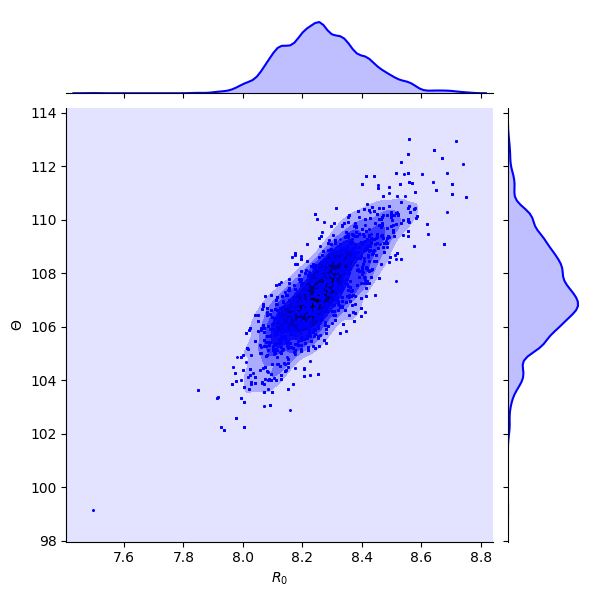
\includegraphics[width=0.9\textwidth]{../../sources/scripts/out.png}
\pagebreak

\subsubsection{Обобщение результатов}
\paragraph{Проверка остатков модели на нормальность.}
\par Для проверки того, что невязки распределены нормально, использовался критерий Шапиро-Уилка \cite{33}. Результаты приведены в таблице.
\begin{figure}[h!]
        \caption{Распределение остатков $\Delta_{\Theta} = \Theta_{\mathr{mod}} - \Theta_{\mathrm{obs}}.}
\begin{minipage}[h]{1\linewidth}
        \includegraphics[width=0.95\textwidth]{../../build/find_sigma_0_no_except/1/theta_err.png}
\end{minipage}
\end{figure}


\pagebreak


% У заключения нет номера главы
\section*{Заключение}
\setmonofont[Mapping=tex-text]{CMU Typewriter Text}
\pagebreak
\bibliography{diploma.bib}
\bibliographystyle{ugost2008ls}
\end{document}
